% Basic stuff
\documentclass[a4paper,10pt]{article}
\usepackage[nswissgerman]{babel}

% 3 column landscape layout with fewer margins
\usepackage[landscape, left=0.75cm, top=1cm, right=0.75cm, bottom=1.5cm, footskip=15pt]{geometry}
\usepackage{flowfram}
\ffvadjustfalse
\setlength{\columnsep}{1cm}
\Ncolumn{3}

% define nice looking boxes
\usepackage[many]{tcolorbox}

% a base set, that is then customised
\tcbset {
  base/.style={
    boxrule=0mm,
    leftrule=1mm,
    left=1.75mm,
    arc=0mm, 
    fonttitle=\bfseries, 
    colbacktitle=black!10!white, 
    coltitle=black, 
    toptitle=0.75mm, 
    bottomtitle=0.25mm,
    title={#1},
    breakable
  }
}

\definecolor{analysis-ii}{rgb}{0.85, 0.24, 0.20}
\newtcolorbox{mainbox}[1]{
  colframe=analysis-ii, 
  base={#1}
}

\newtcolorbox{subbox}[1]{
  colframe=black!20!white,
  base={#1}
}

% Mathematical typesetting & symbols
\usepackage{amsthm, mathtools, amssymb} 
\usepackage{marvosym, wasysym}
\usepackage{derivative}
\allowdisplaybreaks

% Tables
\usepackage{tabularx, multirow}
\usepackage{booktabs}

% Make enumerations more compact
\usepackage{enumitem}
\setitemize{itemsep=0.5pt}
\setenumerate{itemsep=0.75pt}

% To include sketches & PDFs
\usepackage{graphicx}

% For hyperlinks
\usepackage{hyperref}
\hypersetup{
  colorlinks=true
}

% No newline after subsubsections
\usepackage[compact]{titlesec}
\titleformat{\subsubsection}[runin]{\bfseries}{}{0pt}{}[]

% Nice quotes
\usepackage{dirtytalk}

% Metadata
\title{Cheatsheet Analysis II}
\author{Julian Steinmann}
\date{Wintersession 2023}

% Math helper stuff
\def\limn{\lim_{n\to \infty}}
\def\limxo{\lim_{x\to 0}}
\def\limxi{\lim_{x\to\infty}}
\def\limxn{\lim_{x\to-\infty}}
\def\sumk{\sum_{k=1}^\infty}
\def\sumn{\sum_{n=0}^\infty}
\def\R{\mathbb{R}}
\def\C{\mathbb{C}}
\def\Q{\mathbb{Q}}
\def\N{\mathbb{N}}
\def\X{\mathcal{X}}
\def\dx{\; \mathrm{d}x}
\def\smallCalO{\begin{smallmatrix}\!\mathcal{O}\!\end{smallmatrix}}  % Ugly, but Wikipedia does it too...
\DeclareMathOperator{\gradient}{grad}
\DeclareMathOperator{\divergence}{div}
\DeclareMathOperator{\trace}{spur}
\DeclareMathOperator{\curl}{curl}
\DeclareMathOperator{\Hess}{Hess}
\DeclarePairedDelimiter\abs{\lvert}{\rvert}
\DeclarePairedDelimiter\norm{\lVert}{\rVert}


\begin{document}


\section{Gewöhnliche Differentialgleichungen (ODEs)}

\subsection{ODE}

\begin{mainbox}{}
    Eine Gleichung der Form \( G(y, y', \dots, y^{(k)}, x) = 0 \) heisst \emph{gewöhnliche Differentialgleichung \( k \)-ter Ordnung} (engl. ODE). Eine \emph{Lösung} ist eine \( k \)-mal differenzierbare Funktion \( f: \: I \to \R \) auf einem offenen Intervall \( I \subseteq \R \) mit
    \[ G(f(x), f'(x), \dots, f^{(k)}(x), x) = 0 \quad \text{für alle \(x \in I\).} \]
    Ist zusätzlich \( {y(x_0) = y_0}, \, {y'(x_0) = y_1}, \, \dots, \, {y^{(k - 1)}(x_0) = y_{k - 1}} \) mit \( x_0, y_0, y_1, \dots, y_{k - 1} \in \R \) vorgegeben, spricht man von einem \emph{Anfangswertproblem}.
\end{mainbox}

\( k \geq 1 \) heisst \emph{Ordnung} der ODE. Dabei gehen wir davon aus, dass \( k \) minimal ist, d.h. dass \( G \) tatsächlich von \( y^{(k)} \) abhängt. Eine Gleichung der Form \( G(y, x) = 0 \) ist keine ODE.


\subsection{Separation der Variablen}

\begin{align*}
    &\text{ODE der Form } y' = \frac{1}{a(y)} b(x) \quad \text{für \(a, b\) stetig, \(a(y) \neq 0\)} \\
    \iff & a(y) y' = b(x) \\
    \iff & \int a(y) y'(x) \dx = \int b(x) \dx + c \\
    \iff & A(y) = B(x) + c \quad \text{für Stammfunktionen \(A, B\) von \(a, b\).}
\end{align*}

Es folgt \( y = A^{-1}(B(x) + c) \), falls ein Inverses \( A^{-1} \) existiert.


\subsection{Existenz- und Eindeutigkeitssatz}

\begin{mainbox}{Existenz- und Eindeutigkeitssatz (Satz 2.1.6)}
    Ein Anfangswertproblem erster Ordnung \( y' = F(y, x), \, y(x_0) = y_0 \) mit F stetig differenzierbar hat eine eindeutige \emph{maximale} Lösung.
\end{mainbox}

\underline{Genauer:} Ist \( F: \: \R^2 \to \R \) in einer Umgebung von \( (y_0, x_0) \) stetig, und stetig differenzierbar nach \( y \), dann gibt es eine Lösung \( f: \: I \to \R \) auf einem offenen Intervall \( I \subseteq \R \) mit \( x_0 \in I \), sodass für jede Lösung \( g: \: J \to \R \) gilt: \( J \subseteq I \) und \( f|_J = g \).

Eine ODE von Ordnung \( k \geq 2 \) lässt sich als System von \( k \) ODEs von Ordnung \( 1 \) in \( k \) unbekannten Funktionen \( z_0, \dots, z_{k - 1} \) umschreiben, z. B.: Die Lösungen von \( \exp(y'' y' + \sin(y^{x + 1})) = 3 \) entsprechen denen von
\[ \left| \begin{aligned}
    \exp(z_1' z_1 + \sin(z_0^{x + 1})) &= 3 \\
    z_0' &= z_1
\end{aligned} \right| \]
via \( z_0 = y, \, z_1 = y' \).

Versionen des Existenz- und Eindeutigkeitssatzes gelten auch für Systeme von ODEs, und für ODEs von Ordnung \( \geq 2 \).


\subsection{Lineare ODE}

\begin{mainbox}{(Definition 2.2.1)}
    Eine \emph{lineare ODE} von Ordnung \( k \geq 1 \) ist eine Gleichung
    \begin{equation} \label{script_eq_2}
        y^{(k)} + a_{k - 1} y^{(k - 1)} + \dots + a_0 y = b
    \end{equation}
    wobei die \emph{Koeffizienten} \( a_0, \dots, a_{k - 1} \) und die \emph{Inhomogenität} \( b \) Funktionen \( I \to \C \) sind für ein offenes Intervall \( I \subseteq \R\).
    Eine \emph{Lösung} ist ein \( k \)-mal differenzierbares \( f: \: I \to \C \) mit
    \[ f^{(k)}(x) + a_{k - 1}(x) y^{(k - 1)}(x) + \dots + a_0(x) y(x) = b(x) \]
    für alle \( x \in I \). (Wobei \( f'(x) = (\Re(f(x)))' + i (\Im(f(x)))' \)).
    Falls \( b = 0 \), nennen wir \eqref{script_eq_2} \emph{homogen}, sonst \emph{inhomogen}.
    Die Gleichung
    \begin{equation} \label{script_eq_3}
        y^{(k)} + a_{k - 1} y^{(k - 1)} + \dots + a_0 y = 0
    \end{equation}
    heisst die \emph{zu \eqref{script_eq_2} gehörige homogene lineare ODE}.
\end{mainbox}

Falls \( a_i, b \) reellwertig, dann suchen wir meist reellwertige Lösungen.

Sind \( f_1, f_2 \) Lösungen einer homogenen linearen ODE, dann ist es auch \( \lambda f_1 + f_2 \) für \( \lambda \in \C \).

\begin{subbox}{(Satz 2.2.3)}
    Annahme: \( a_0, \dots, a_{k - 1}, b \) stetig.
    \begin{itemize}
        \item Die Lösungen der \emph{homogenen} linearen ODE \eqref{script_eq_3} bilden einen \( \C \)-Vektorraum \( S \) mit \( \dim S = k \).
        \item Die \emph{inhomogene} lineare ODE \eqref{script_eq_2} hat eine Lösung \( f_0 \). Die Menge aller Lösungen von \eqref{script_eq_2} ist genau der affine Raum \( f_0 + S \).
        \item Für beliebige \( x_0 \in I, \quad y_0, \dots, y_{k - 1} \in \C \) hat das \emph{Anfangswertproblem} \eqref{script_eq_2} mit \( y(x_0) = y_0, \dots, y^{(k - 1)}(x_0) = y_{k - 1} \) genau eine Lösung.
        \item \( a_0, \dots, a_{k - 1}, b \text{ \emph{reellwertig}}  \implies \dim_\R \{ \text{reellwertige } f \in S \} = k \), \eqref{script_eq_2} hat eine reellwertige Lösung \( f_0 \), und \( \{ \text{reellwertige Lösungen von \eqref{script_eq_2}} \} = f_0 + \{ \text{reellwertige } f \in S \} \). Für \( x_0 \in I, \, y_0, \dots, y_{k - 1} \in \R \) hat das entsprechende Anfangswertproblem genau eine Lösung.
    \end{itemize}
\end{subbox}

\subsubsection{Lösungsstrategie für lineare ODE}
\begin{enumerate}
    \item Finde Basis \( f_1, \dots, f_k \) des Lösungsraums \( S \) der \emph{homogenen} ODE. (\( k = 1 \): Finde eine nicht-triviale Lösung \( f_1 \).)
    \item Finde eine einzelne Lösung \( f_0 \) der \emph{inhomogenen} ODE (\say{Partikulärlösung}). Die allgemeine Lösung ist \( f_0 + \sum_{i = 1}^k \lambda_i f_i, \quad \lambda_i \in \R \text{ oder } \C \). (\( k = 1 \): \(f_0 + \lambda_1 f_1 \))
    \item Einsetzen der Anfangswerte in die allgemeine Lösung \( \rightarrow \) lineares Gleichungssystem für \( \lambda_1, \dots, \lambda_k \) mit eindeutiger Lösung. (\( k = 1 \): Eine einzelne lineare Gleichung \( f_0(x_0) + \lambda_1 f_1(x_0) = b(x_0) \).
\end{enumerate}


\subsection{Lineare ODE erster Ordnung}

\underline{Zu lösen:} \( y' + ay = b \) mit gegebenen stetigen \( a, b: \: I \to \C \).

\begin{subbox}{(Proposition 2.3.1)}
    Die Lösungen von \( y' + ay = 0 \) sind genau \( f(x) = z e^{-A(x)} \), für \( A \) eine Stammfunktion von \( a \) und \( z \in \C \).
\end{subbox}

\begin{proof}
    Dass \( z e^{-A(x)} \) eine Lösung ist, lässt sich einfach nachrechnen. Dass alle Lösungen von dieser Form sind, folgt daraus, dass sie nach Satz 2.2.3 einen eindimensionalen Vektorraum bilden.
    Ein alternativer Beweis dafür: sei \( f \) eine Lösung. Wähle \( x_0 \in I \) und setze \( z = f(x_0) e^{A(x_0)} \). Dann \( f(x_0) = z e^{-A(x_0)} \). Nun sind \( f \) und \( z e^{-A(x_0)} \) zwei maximale Lösungen des Anfangswertproblems \( y' + ay = 0, \quad y(x_0) = f(x_0) \). Nach dem Existenz- und Eindeutigkeitssatz folgt \( f(x) = z e^{-A(x)} \) für alle \( x \in I \).
\end{proof}

Herleiten lässt sich die Formel \( z e^{-A(x)} \) durch Separation der Variablen.

\subsection{Lineare ODE mit konstanten Koeffizienten}

\begin{equation} \label{script_eq_4}
    y^{(k)} + a_{k - 1} y^{(k - 1)} + \dots + a_0 y = b, \quad a_0, \dots, a_{k - 1} \in C
\end{equation}

\subsubsection{Lösung der homogenen ODE}
\underline{Ansatz:} \( f(x) = e^{\alpha x} \)? Einsetzen:
\begin{align*}
    & \alpha^k e^{\alpha x} + a_{k - 1} \alpha^{k - 1} e^{\alpha x} + \dots + a_0 e^{\alhpha x} = 0 \\
    \iff & \alpha^k + a_{k - 1} \alpha^{k - 1} + \dots + a_0 = 0 \\
    \iff & \alpha \text{ Nullstelle von \( P(t) \), wobei:}
\end{align*}

\begin{mainbox}{Charakteristisches Polynom}
    \( P(t) = t^k + a_{k -1} t^{k - 1} + \dots + a_0 \) heisst \emph{charakteristisches Polynom} der ODE \eqref{script_eq_4}.
\end{mainbox}

\begin{subbox}{}
    Ist \( \alpha \) eine Nullstelle von \( P \), so löst \( e^{\alpha x} \) die homogene ODE \eqref{script_eq_4}. Hat \( P \) keine mehrfachen Nullstellen, ist \( \{ e^{\alpha x} \; | \; \alpha \in \C, \, P(\alpha) = 0 \} \) eine Basis des Lösungsraums \( S \).
\end{subbox}

\begin{proof}
    Fundamentalsatz der Algebra \( \implies \) Falls \( P \) keine mehrfachen Nullstellen hat, so hat \( P \) \( k \) viele Nullstellen \( \alpha_1, \dots, \alpha_k \). Dann sind \( e^{\alpha_1 x}, \dots, e^{\alpha_k x} \) linear unabhängige Funktionen \( \R \to \C \). Da \( \dim S = k \) nach Satz 2.2.3, ist \( e^{\alpha_1 x}, \dots, e^{\alpha_k x} \) eine Basis.
\end{proof}

\begin{subbox}{}
    Hat \( P \) Nullstellen \( \alpha_1, \dots, \alpha_l \) mit Vielfachheiten \( v_1, \dots, v_l \), ist eine Basis des Lösungsraums \( \{ x^j e^{\alpha_i x} \; | \; i \in \{ 1, \dots, l \}, \, j \in \{0, \dots, v_i - 1 \} \} \).
\end{subbox}

Falls \( a_0, \dots, a_{k - 1} \in \R \), so ist \( \alpha = \beta + i \gamma \) Nullstelle von \( P \) genau dann wenn \( \bar{\alpha} = \beta - i \gamma \) Nullstelle ist. Nun findet man eine reellwertige Basis des Lösungsraums indem man \( e^{\alpha x}, e^{\bar{\alpha} x} \) durch \( e^{\beta x} \cos(\gamma x), \, e^{\beta x} \sin(\gamma x) \) ersetzt.

\begin{subbox}{Superpositionsprinzip (2.2.5)}
    Löst \( f_0 \) die ODE mit inhomogenem Term b und \( g_0 \) die ODE mit inhomogenem Term \( c \), so löst \( \lambda f_0 + \mu g_0 \) die ODE mit inhomogenem Term \( \lambda b + \mu c \).
\end{subbox}

\subsubsection{Methode der unbestimmten Koeffizienten}
Ansatz: Eine Lösung suchen, die \say{ähnlich aussieht} wie \( b \). Tatsächlich gilt:

\begin{itemize}
    \item \( b(x) = x^d e^{\beta x} \) \( \implies \) \eqref{script_eq_4} hat Lösung der Form \( Q(x) e^{\beta x} \), für ein Polynom \( Q \) von Grad \( \leq d \) (falls \( P(\beta) \neq 0 \)), bzw. von Grad \( \leq d + j \) (falls \( \beta \) \( i \)-fache Nullstelle von P).
    \item \( b(x) = x^d \cos(\beta x) \) oder \( x^d \sin(\beta x) \) \( \implies \) \eqref{script_eq_4} hat Lösung der Form \( Q_1(x) \cos(\beta x) + Q_2(x) \sin(\beta x) \), mit \( Q_1, Q_2 \) wie im ersten Punkt \( Q \)
\end{itemize}

Im 2. Fall \( b(x) = x^d \cos(\beta x) \) oder \( x^d \sin(\beta x) \) muss man prüfen, ob \( \beta_i \) (nicht \( \beta \) wie im 1. Fall) eine \( j \)-fache Nullstelle von \( P \) ist. Die Polynome \( Q_1, Q_2 \) haben dann Grad \( \leq d + j \).


\subsection{Harmonischer Oszillator}

\[ y(x) = \text{Auslenkung des Körpers zum Zeitpunkt \( x \)} \]
Dann gilt die ODE
\[ my'' = -by' - ky \]
wobei \( m \) die Masse, \( b \geq 0 \) der Widerstand, \( k > 0 \) die Federkonstante. \\
Falls \( b = 0 \), sind alle Lösungen periodisch. \\
Falls \( b > 0 \), gilt für alle Lösungen \( \limxi y(x) = 0 \). \\
Für \( b^2 - 4km > 0 \) findet man eine oszillierende Lösung. \\
Für \( b^2 - 4km \leq 0 \) hingegen eine nicht oszillierende Lösung. \\


\subsection{Variation der Konstanten}

\underline{Zu lösen:} \( y' + ay = b \). Ansatz: \( f(x) = z(x) e^{-A(x)} \).
In ODE einsetzen:
\begin{align*}
    & f'(x) + a(x) f(x) = b(x) \\
    \iff & z'(x) e^{-A(x)} - z(x) a(x) e^{-A(x)} + a(x) z(x) e^{-A(x)} = b(x) \\
    \iff & z'(x) e^{-A(x)} = b(x) \\
    \iff &z'(x) = e^{A(x)} b(x)
\end{align*}

Wähle für \( z \) eine Stammfunktion von \( e^{A(x)} \) b(x).
Dann ist \( f(x) = z(x) e^{-A(x)} \) eine Lösung.
Falls \( y(x_0) = y_0 \) gegeben, wähle die Stammfunktion so, dass \( z(x_0) e^{-A(x_0)} = y_0 \).

\subsubsection{Variation der Konstanten für Ordnung \( \geq 2 \)}
Spezialfall ODE zweiter Ordnung
\[ y'' + a_1 y' + a_0 y = b \]
Erst Basis \( f_1, f_2 \) des Lösungsraumes der homogenen ODE finden. \\
Ansatz:
\[ \left| \begin{aligned}
    z_1(x) f_1(x) + z_2(x) f_2(x) &= f_0(x) \\
    z_1'(x) f_1(x) + z_2'(x) f_2(x) &= 0
\end{aligned} \right| \]
Berechne:
\begin{align*}
    f_0' &= z_1' f_1 + z_1 f_1' + z_2' f_2 + z_2 f_2' \\
    &= z_1 f_1' + z_2 f_2'
\end{align*}
\[ f_0'' &= z_1' f_1' + z_1 f_1'' + z_2' f_2' + z_2 f_2'' \]
In ODE einsetzen:
\begin{align*}
    b &= z_1(\underbrace{f_1'' + a_1 f_1' + a_0 f_0}_{= 0}) \\
    &+ z_2(\underbrace{f_2'' + a_1 f_2' + a_0 f_2}_{= 0}) \\
    &+ z_1' f_1' + z_2' f_2'
\end{align*}
Also:
\begin{align*}
    & f_0 \text{ Lösung} \\
    \iff & \left| \begin{aligned}
        z_1' f_1 + z_2' f_2 &= 0 \\
        z_1' f_1' + z_2' f_2' &= b
    \end{aligned} \right| \\
    \iff & \underbrace{\begin{pmatrix*}
        f_1 & f_2 \\
        f_1' & f_2'
    \end{pmatrix*}}_A \begin{pmatrix*}
        z_1' \\ z_2'
    \end{pmatrix*} = \begin{pmatrix*}
        0 \\ b
    \end{pmatrix*} \\
    \implies & \begin{pmatrix*}
        z_1' \\ z_2'
    \end{pmatrix*} = A^{-1} \begin{pmatrix*}
        0 \\ b
    \end{pmatrix*}
\end{align*}

Dies sind explizite Formeln für \( z_1', z_2' \). Schliesslich nach Stammfunktion von \( z_1', z_2' \) finden.


\section{Differentialrechnung in \(\R^n\)}

\[ f: \: \R^n \to \R^m \]


\subsection{Stetigkeit und Konvergenz im Mehrdimensionalen}

Die \emph{Norm} von \( x \in \R^n \) ist \( \norm{x} = \sqrt{x_1^2 + \dots + x_n^2} \).

\begin{mainbox}{Stetigkeit (Definition 3.2.3)}
    \( U \subseteq \R^n \), \( f: \: x \to \R^m \) heisst \emph{stetig bei \( x_0 \in U \)} falls für alle \( \varepsilon > 0 \) existiert \( \delta > 0 \) sodass \( \norm{x - x_0} < \delta \implies \norm{f(x) - f(x_0)} < \varepsilon \). \( f \) heisst \emph{stetig} falls \( f \) bei allen \( x_0 \in U \) stetig ist.
\end{mainbox}

\begin{mainbox}{Konvergenz (Definition 3.2.1)}
    Eine Folge \( x_1, x_2, \dots \in \R^n \) \emph{konvergiert gegen \( y \in \R^n \)} (geschrieben \( \limxi x_k = y \)) falls für  alle \( \varepsilon > 0 \) existiert \( N \) sodass für alle \( k \geq N \) gilt: \( \norm{x_k - y} < \varepsilon \).
\end{mainbox}

\begin{subbox}{(Lemma 3.2.2)}
    \begin{align*}
        & \underbrace{\lim_{k \to \infty}}_\text{Limes in \( \R^n \)} x_k = y \\
        \iff & \underbrace{\lim_{k \to \infty}}_\text{Limes in \( \R \)} \norm{x_k - y} = 0 \\
        \iff & \underbrace{\lim_{k \to \infty}}_\text{Limes in \( \R \)} x_{k, l} = y_l \quad \text{für alle \( l \in \{ 1, \dots, n \} \)}
    \end{align*}
\end{subbox}

\begin{subbox}{(Satz 3.2.4)}
    \( U \subseteq \R^n \), \( f: \: U \to \R^m \) ist stetig bei \( x_0 \in U \) \( \iff \) falls \( x_1, x_2, \dots \in U \) mit \( \lim_{k \to \infty} x_k = x_0 \), dann \( \lim_{k \to \infty} f(x_k) = f_(x_0) \).
\end{subbox}

\begin{subbox}{(Satz 3.2.9)}
    \( f: \: \underbrace{U}_{\in \R^n} \to \underbrace{V}_{\in \R^m} \) und \( g: \: V \to \R^p \) stetig \( \implies \) \(g \circ f \) stetig.
\end{subbox}

\begin{proof}
    Mit Satz 3.2.4. Falls \( x_1, x_2, \dots, \in U \) konvergiert, dann
    \[ g(f(\lim_{k \to \infty} x_k)) = g(\lim_{k \to \infty} f(x_k)) = \lim_{k \to \infty} g(f(x_k)) \]
    Die erste Gleichheit gilt weil \( f \) stetig ist, die zweite weil \( g \) stetig ist.
\end{proof}

\begin{subbox}{(Definition 3.2.5}
    \( U \subseteq \R^n \), \(f: \: U \to \R^m \). Der \emph{Grenzwert von \( f \) bei \( x_0 \in U \)} ist gleich \( y \in \R^m \), geschrieben \( \lim_{x \to x_0, \, x \neq x_0} f(x) = y \), falls für alle \( \varepsilon > 0 \) ein \( \delta > 0 \) existiert, sodass \( x \in U \) mit \( \norm{x - x_0} < \delta \) und \( x \neq x_0 \) \( \implies \) \( \norm{f(x) - y} < \varepsilon \).
\end{subbox}

Der Wert \( f(x_0) \) hat keinen Einfluss auf \( \lim_{x \to x_0, \, x \neq x_0} f(x) \).

\begin{subbox}{(Satz 3.2.7)}
    \( \lim_{x \to x_0, \, x \neq x_0} f(x) = y \) \( \iff \) für jede Folge \( x_1, x_2, \dots \in U \) mit \( \lim_{k \to \infty} x_k = x_0 \) und \( x_k \neq x_0 \) gilt \( \lim_{k \to \infty} f(x_k) = y \).
\end{subbox}

\begin{mainbox}{(Definition 3.2.11)}
    \( U \subseteq \R^n \) heisst:
    \begin{itemize}
        \item \emph{beschränkt} falls \( \{ \norm{x} \; | \; x \in U \} \) beschränkt
        \item \emph{abgeschlossen} falls \( x_1, x_2, \dots \in U \), \( \lim_{k \to \infty} x_k = y \implies y \in U \)
        \item \emph{offen} falls für alle \( x \in U \) existiert \( \delta > 0 \) sodass \[ \{ y \in R \; | \; \abs{x_i - y_i} < \delta \text{ für alle } i \} \subseteq U \]
        \item \emph{kompakt} falls \( U \) abgeschlossen und beschränkt ist.
    \end{itemize}
\end{mainbox}

\begin{subbox}{(Satz 3.3.2)}
    \( U \subseteq \R^n \) offen \( \iff \) \(\R^n \setminus U \) abgeschlossen.
\end{subbox}

\begin{subbox}{(Satz 3.2.13)}
    \( f: \: \R^n \to \R^m \) stetig. Dann:
    \begin{enumerate}
        \item \( V \subseteq \R^m \) abgeschlossen \( \implies \) \( f^{-1}(V) \subseteq \R^n \) abgeschlossen
        \item \( V \subseteq \R^m \) offen \( \implies \) \( f^{-1}(V) \subseteq \R^n \) offen
    \end{enumerate}
    Hier ist \( f^{-1}(V) \) das \emph{Urbild von \( V \) bezüglich \( f \)}, d.h. \( f^{-1}(V) = \{ x \in \R^n \; | \; f(x) \in V \} \). Dies ist für alle \( f: \: \R^n \to \R^m \) definiert, auch solche \( f \), die keine Umkehrfunktion \( f^{-1} \) haben.
\end{subbox}

\begin{proof}
    \begin{enumerate}
        \item \( x_1, x_2, \dots \in f^{-1}(V) \) und \( \lim_{k \to \infty} x_k = y \) \( \implies \) \( f(y) \in V \implies y \in f^{-1}(V) \).
        \item \( V \) offen \( \implies \) \( \R^m \setminus V \) abgeschlossen \( \implies \) \( \underbrace{f^{-1}(\R^m \setminus V)}_{\R^m \setminus f^{-1}(V)} \) abgeschlossen \( \implies \) \( f^{-1}(V) \) offen.
    \end{enumerate}
\end{proof}

\begin{subbox}{(Satz 3.2.15)}
    \( U \in \R^n \) nicht-leer und kompakt, \( f: \: U \to \R \) stetig \( \implies \) \( f \) ist beschränkt und nimmt ein Minimum und ein Maximum an, d.h. es gibt \( x_+, x_- \in U \) sodass \( f(x_+) = \sup_{x \in U} f(x), \, f(x_-) = \inf_{x \in U} f(x) \).
\end{subbox}


\subsection{Partielle Ableitungen}

\begin{mainbox}{Partielle Ableitung (Definition 3.3.5)}
    \( U \subseteq \R^m \) offen, \( f: \: U \to \R \). Die \emph{\( i \)-te partielle Ableitung von \( f \) bei \( x_0 \in U \)} ist \( \partial_{x_i} f \coloneqq g'(x_{0, i}) \in \R \), wobei \( g: \: \{ t \in \R \; | \; (x_{0, 1}, \dots, \underbrace{t}_\text{Index \( i \)}, \dots, x_{0, n}) \in U \} \to \R \), \( g(t) = f(x_{0, 1}, \dots, \underbrace{t}_\text{Index \( i \)}, \dots, x_{0, n}) \), falls \( g \) bei \( x_0 \) differenzierbar.
\end{mainbox}

Andere Schreibweisen:
\[ \partial_{x_i} f = \partial_i f = \frac{\partial f}{\partial x_i} = f_{x_i} \]

Falls \( \partial_{x_i} \) überall existiert, ist \( \partial_{x_i} f \) selbst wieder eine Funktion \( U \to \R^m \), genau wie \( f \). Also kann man höhere partielle Ableitung betrachten: \( \partial_{x_j} \partial_{x_i} f \). Andere Notationen:
\[ \partial_{ji} f = \frac{\partial^2 f}{\partial x_j \, \partial x_i} = f_{x_j x_i} \]

\begin{mainbox}{Jacobimatrix (Definition 3.3.9)}
    \( U \subseteq \R^n \) offen, \( f: \: U \to \R^m, \ f = (f_1, \dots, f_m) \) mit \( f_i: \: U \to \R \).
    Die \( m \! \times \! n \)-Matrix
    \[ J_f(x) = \left( \partial_j f_i(x) \right)_\substack{1 \leq i \leq m \\ 1 \leq j \leq n} \]
    heisst \emph{Jacobimatrix von \( f \) bei \( x \)}.
\end{mainbox}

\begin{mainbox}{Gradient, Divergenz (Definition 3.3.11)}
    \( U \subseteq \R^m \) offen
    
    Der \emph{Gradient} von \( f: \: U \to \R \) bei \( x_0 \in U \) ist
    \[ \gradient f(x_0) = \nabla f(x_0) = \begin{pmatrix*}
        \partial_1 f(x_0) \\
        \vdots \\
        \partial_n f(x_0)
    \end{pmatrix*} = J_f(x_0)^\mathrm{T} \]

    Die \emph{Divergenz} von \(f: \: U \to \R^n \) bei \( x_0 \in U \) ist
    \[ \divergence f(x_0) = \partial_1 f_1(x_0) + \dots + \partial_n f_n(x_0) = \trace J_f(x_0) \]
\end{mainbox}


\subsection{Differential}

Für Funktionen \( f: \: \R \to \R \) bedeutet Differenzierbarkeit bei \( x_0 \), dass \( f \) in der Nähe von \( x_0 \) gut durch eine Gerade angenähert wird.

Entsprechend definieren wir, dass \( f: \: \R^n \to \R^m \) bei \( x_0 \in \R^n \) differenzierbar ist, wenn \( f \) in der Nähe von \( x_0 \) gut durch eine affine Funktion (= Konstante + lineare Funktion) angenähert wird.

\begin{mainbox}{Differenzierbarkeit, Differenzial (Definition 3.4.2)}
    \( U \subseteq \R \) offen, \( f: \: U \to \R^m \), \( A \) eine lineare Abbildung \( \R^n \to \R^m \). \( f \) heisst \emph{differenzierbar bei \( x_0 \in U \) mit Differential \( A \)}, geschrieben \( \mathrm{d} f(x_0) = A \), falls
    \[ \lim_{x \to x_0, \, x \neq x_0} \frac{f(x) - f(x_0) - A (x - x_0)}{\norm{x - x_0}} = 0 \]
\end{mainbox}

\( \mathrm{d} f(x_0) = A \) \( \iff \) \( f \) hat die \emph{Dreigliedentwicklung}
\[ f(x) = f(x_0) + A(x - x_0) + \text{Fehler}(x - x_0) \]
wobei \( \text{Fehler}(x - x_0) = \smallCalO (\norm{x - x_0}) \), d.h.
\[ \lim_{x \to x_0, \, x \neq x_0} \frac{\text{Fehler}(x - x_0}{\norm{x - x_0}} = 0 \]

Für \( f: \: \R \to \R \) ist \( \mathrm{d} f(x_0) \) die lineare Abbildung \( \R \to \R, \, x \mapsto f'(x_0) \cdot x \).

\( f = (f_1, \dots, f_m \) differenzierbar \( \iff \) \( f_1, \dots, f_m \) differenzierbar

\begin{subbox}{Stetige Differenzierbarkeit (Satz 3.4.7)}
    \( U \subseteq \R^n \) offen, \(f: \: U \to \R^m \). Falls \( \partial_{xj} f_i \) für alle \( 1 \leq j \leq m, \, 1 \leq i \leq m \) existiert und stetig ist, dann ist \( f \) differenzierbar.
    Wir nennen \( f \) dann \emph{stetig differenzierbar}.
\end{subbox}

\begin{subbox}{(Satz 3.4.4)}
    \( U \subseteq \R^n \) offen, \( f: \: U \to \R^m \) differenzierbar. Dann
    \begin{itemize}
        \item \( f \) ist stetig.
        \item \( \partial_{xj} f_i \) existiert für \( 1 \leq j \leq n, \, 1 \leq i \leq m \).
        \item Die Matrix von \( \mathrm{d} f (x_0) \) bezüglich den Standardbasen von \( \R^n, \R^m \) ist gleich \( J_f(x_0) \).
    \end{itemize}
\end{subbox}

\begin{subbox}{(Satz 3.4.6)}
    \( U \subseteq \R^n \) offen, \(f, g: \: U \to \R^m \) differenzierbar. Dann:
    \begin{itemize}
        \item \( f + g \) ist differenzierbar und \( \mathrm{d} (f + g)(x_0) = \mathrm{d} f(x_0) + \mathrm{d} y(x_0) \).
        \item \( m = 1 \) \( \implies \) \( fg \) ist differenzierbar.
        \item \( m = 1, \, g \neq 0 \) \( \implies \) \( \frac{f}{g} \) ist differenzierbar.
    \end{itemize}
\end{subbox}

\begin{subbox}{Kettenregel (Satz 3.4.9)}
    \( U \subseteq \R^n \) offen, \( V \subseteq \R^m \) offen, \( f: \: U \to V, \, g: \: V \to \R^p \) differenzierbar. Dann ist \( g \circ f \) differenzierbar und
    \[ \mathrm{d} (g \circ f)(x_0) = \mathrm{d} g(f_(x_0)) \circ \mathrm{d} f(x_0) \]
    Insbesondere erfüllen die Jacobimatrizen
    \[ J_{g \circ f}(x_0) = J_g(f(x_0)) J_f(x_0) \]
\end{subbox}

Falls \( p = 1 \), kann man die Kettenregel auch mit Gradienten schreiben:
\[ \nabla_{g \circ f} = J_{g \circ f}^\mathrm{T}, \quad \nabla_g = \nabla_g^\mathrm{T} \]
also
\[ \underbrace{\nabla_{g \circ f}(x_0)}_{\in \R^n} = \underbrace{J_f(x_0)^\mathrm{T}}_{\in \R^{n \! \times \! m}} \cdot \underbrace{\nabla_g(f(x_0))}_{\in \R^m} \]


\subsection{Tangentialraum und Richtungsableitungen}

\begin{mainbox}{Tangentialraum (Definition 3.4.11)}
    \( U \subseteq \R^n \) offen, \( f: \: U \to \R^m \) differenzierbar, \( x_0 \in U \), \( A = \mathrm{d} f(x_0) \). Der \emph{Tangentialraum bei \( x_0 \) des Graphen von \( f \)} ist der Graph von \( g(x) = f(x_0) + A(x - x_0) \), also \( \{ (x, g(x)) \; | \; x \in \R^n \} \subseteq \R^n \times \R^m \).
\end{mainbox}

\begin{subbox}{Richtungsableitung (Definition 3.4.13)}
    \( U \subseteq \R^n \) offen, \(f: \: U \to \R^m \), \( v \in \R^n \setminus \{ 0 \} \), \(x_0 \in U \). Die \emph{Richtungsableitung von \( f \) in Richtung \( v \) bei \( x_0 \)} ist \( D_v f(x_0) \coloneqq \underbrace{J_g(0)}_{\left( \begin{smallmatrix}
        \partial_x g_1(0) \\
        \vdots \\
        \partial_x g_m(0)
    \end{smallmatrix} \right)} \in \R^m \), wobei \( g: \: \{ t \in \R \; | \; x_0 + tv \in U \} \to \R^m, \, g(t) = f(x_0 + tv) \).
\end{subbox}

Falls \( m = 1\), dann \( D_{e_i} f(x_0) = \partial_{x_i} f(x_0) \) für \( e_i \) den \( i \)-ten Standardbasisvektor.

\begin{subbox}{(Satz 3.4.15)}
    \( U \subseteq \R^n \) offen, \( f: \: U \to \R^m \) stetig differenzierbar \( \implies \) für alle \( x_0 \in U, \, v \in \R^n \setminus \{ 0 \} \) gilt \(D_v f(x_0) = \mathrm{d} f(x_0)(v) \). Insbesondere
    \[ D_{\lambda_1 v_1 + \lambda_2 v_2} f(x_0) = \lambda_1 D_{v_1} f(x_0) + \lambda_2 D_{v_2} f(x_0) \]
\end{subbox}


\subsection{Höhere Ableitungen}

\begin{mainbox}{(Definition 3.5.1)}
    \begin{align*}
        C^0(U, \R^m) &\coloneqq \{ \text{stetige Funktionen } f: \: U \to \R^m \} \\
        \underbrace{C^k(U, \R^m)}_\text{für \( k \geq 1 \)} &\coloneqq \{ f \text{ diffbar und alle } \partial_{x_j} f \in C^{k - 1}(U, \R^m) \} \\
        &= \{ f \text{ sodass alle } \partial_{x_{j_1}}, \dots, \partial_{x_{j_k}} f_i \text{ existieren \& stetig sind} \} \\
        &= \text{\say{\( k \)-mal stetig differenzierbar}} \\
        C^\infty(U, \R^m) &\coloneqq \bigcap_{k = 0}^\infty C^k(U, \R^m) \\
        &= \text{\say{glatt}}
    \end{align*}
    Wir haben \( C^0 \supseteq C^1 \supseteq C^2 \supseteq \dots \supseteq C^\infty \)
\end{mainbox}

\begin{mainbox}{Hessische (Definition 3.5.9)}
    \( U \subseteq \R^n \) offen, \( (f: \: U \to \R) \in C^2 \), \( x_0 \in U \). Die \emph{Hessische von \(f \) bei \( x_0 \)} ist die \( n \! \times \! n \)-Matrix
    \[ H_f(x_0) = (\partial_{x_i} \partial_{x_j} f(x_0))_\substack{1 \leq i \leq n \\ 1 \leq j \leq n} \]
\end{mainbox}

\begin{subbox}{(Satz 3.5.4)}
    \( U \subseteq \R^n \) offen, \( f \in C^2(U, \R^m) \). Dann gilt
    \[ \partial_{x_j} \partial_{x_l} f = \partial_{x_l} \partial_{x_j} f \]
\end{subbox}

\begin{subbox}{}
    Ist \( f \in C^k \), so lassen sich \( \partial_{x_{j_1}}, \dots, \partial_{x_{j_k}} \) beliebig vertauschen!
\end{subbox}


\subsection{Taylorpolynome}

Dreigliedentwicklung von \( f \in C^1(U, \R) \) für \( U \subseteq \R \) offen
\[ f(x) = \underbrace{f(x_0) + f'(x_0) \cdot y}_{T_1 f(x) \text{ (Polynom von Grad \( \leq 1 \))}} + \smallCalO(\abs{y}) \]
wobei \( y = x - x_0 \).

Annäherung durch Taylorpolynome für \( f \in C^k \):
\[ f(x) = \underbrace{\sum_{j = 0}^k \frac{1}{j!} \cdot f^{(j)}(x_0) \cdot y^j}_{T_k f(x) \text{ Polynom von Grad \( \leq k \)}} + \smallCalO(\abs{y}^k) \]

\( T_k f(x) \) ist das einzige Polynom \( P(x) \) von Grad \( \leq k \), sodass \( P(x_0) = f(x_0), \, P'(x_0) = f'(x_0), \, \dots, \, P^{(k)}(x_0) = f^{(k)}(x_0) \).

Erinnerung: \( \deg x_1^{m_1} \cdot \dots \cdot x_n^{m_m} = m_1 + \dots + m_m \)


\subsection{Exkurs zum Landau-Symbol \texorpdfstring{\( \smallCalO \)}{ℴ}}

\begin{mainbox}{}
    \( U \subseteq \R^n \), \( g: \: U \to \R \), \( x_0 \in U \). Dann ist \emph{\( \smallCalO(g) \)} die Menge der Funktionen \( f: \: U \to \R \) mit \( \lim_{x \to x_0, \, x \neq x_0} \abs{\frac{f(x)}{g(x)}} = 0 \) (die Betragsstriche können auch weggelassen werden, das wäre äquivalent).

    Schreibweise: \( f = \smallCalO(g) \) anstatt \( f \in \smallCalO(g) \), \( \smallCalO(f) = \smallCalO(g) \) anstatt \( \smallCalO(f) \subseteq \smallCalO(g) \).

    Für Funktionen \( \R \to \R \), \( x_0 = 0 \) gilt \( x^k = \smallCalO(x^l) \iff k > l \).
\end{mainbox}

\subsubsection{Rechenregeln}
\begin{gather*}
    \smallCalO(x^a) + \smallCalO(x^b) = \smallCalO(x^{\min(a, b)}) \\
    \smallCalO(x^a) \cdot \smallCalO(x^b) = \smallCalO(x^{a + b}) \\
    x^a \smallCalO(x^b) = \smallCalO(x^{a + b})
\end{gather*}
Diese Regeln gelten für \( x_0 = 0 \). Ansonsten muss man \( x \) durch \( y = x - x_0 \) ersetzen.


\subsection{Kritische Punkte}
\subsection{Lagrange-Multiplikatoren}
\subsection{Satz der Umkehrabbildung}
\section{Integration in \(\R^n\)}
\subsection{Wegintegrale}
\subsection{Rotation/Curl}
\subsection{Riemann-Integral in \(\R^n\)}
\subsection{Uneigentliche Integrale}
\subsection{Transformationsformel}
\subsection{Schwerpunktsberechnungen}

\pagebreak
%%% Original cheatsheet below %%%

\maketitle

% Not actually an abstract. We abuse it for licencing
\renewcommand{\abstractname}{Lizenz}
\begin{abstract}
	Dieses Dokument ist unter CC BY-SA 4.0 lizenziert. Es darf verbreitet oder verändert werden, solange der Urheber und die Lizenz erhalten bleibt.

	\begin{center}
		Der \LaTeX-Quelltext ist verfügbar auf \\ \href{https://github.com/XYQuadrat/eth-cheatsheets}{github.com/XYQuadrat/eth-cheatsheets}.
	\end{center}
\end{abstract}


\section{Differentialgleichungen}
\begin{mainbox}{Definition lineare DGL}
  Eine gewöhnliche lineare Differentialgleichung ist eine Gleichung, welche Ableitungen enthält. Sie hat die Form \[y^{(n)} + a_{n-1} y^{(n-1)} + \ldots0 + a_1 y' + a_0y = b(x)\]
  wo die Koeffizienten \(a_0, \ldots, a_{n-1}\) komplexe Funktionen auf \(I \subset \R\) sind, welche von \(y\) abhängig sein können. Wenn \(b(x) = 0\) gilt, ist die DGL homogen.
\end{mainbox}
Die Menge \(S\) an Lösungen ist eine Teilmenge des Raums der komplexen Funktionen auf \(I\) mit Dimension \(n\). \\
\(S_0\) ist die Menge der Lösungen zu einer homogenen DGL. Für ein \(b(x)\) ist die Menge der Lösungen \(S_b = \{f_h + f_p \mid f_h \in S_0\}\).
\subsubsection*{Lineare DGL erkennen}
\begin{itemize}
  \item keine Koeffizienten vor der höchsten Ableitung
  \item alle Koeffizienten sind stetige Funktionen
  \item keine Produkte von $y$ oder deren Ableitungen
  \item keine Potenzen von $y$ oder deren Ableitungen
  \item keine Funktionen von $y$ oder deren Ableitungen
\end{itemize}

\subsection{Lineare DGL erster Ordnung}
Wir betrachten DGL der Form \[y' + a(x)y = b(x)\]
\begin{enumerate}
  \item (Homogene Lösung) 
  \begin{align*}
    y' + a(x)y &= 0\\
    \frac{y'}{y} &= -a(x)\\
    \ln(y) &= -A(x)+C\\
    y &= e^{-A(x)+C} = z \cdot e^{-A(x)}\quad z \in \C
  \end{align*}
  \item (partikuläre Lösung) Verwende entweder ``Variation der Konstanten'' oder ``Fundiertes Raten''.
\end{enumerate}
\subsection{Variation der Konstanten}
Sei \(f_p = z(x)e^{-A(x)}\) für eine Funktion \(z: I \to \C\). Dann ist \(z'(x) = b(x) e^{A(x)}\) und somit \[z(x) = \int_{x_0}^x b(t) e^{A(t)} \mathop{dt}\] Daraus erhalten wir \[f_p = \int_{x_0}^x b(t) e^{A(t)} \mathop{dt} \cdot e^{-A(t)}\]

\subsection{Fundiertes Raten}

Wenn $b(x)$ von einer bestimmten Form ist, versuchen wir folgende $f_p$, wobei wir unseren Versuch in die DGL einsetzen, was uns dann ein Gleichungssystem für die Konstanten gibt:

\begin{center}
  \renewcommand*{\arraystretch}{1.6}
  \begin{tabular}{cc} 
    \toprule
    $b(x)$ & Raten \\ 
    \midrule
    $a \cdot e^{\alpha x}$ & $b \cdot e^{\alpha x}$\\
    $a \sin(\beta x)$ & $c \sin(\beta x) + d \cos(\beta x)$\\
    $b \cos(\beta x)$ & $c \sin(\beta x) + d \cos(\beta x)$\\
    $a e^{\alpha x} \sin(\beta x)$ & $e^{\alpha x} \Big( c \sin(\beta x) + d \cos(\beta x) \Big)$\\
    $b e^{\alpha x} \cos(\beta x)$ & $e^{\alpha x} \Big( c \sin(\beta x) + d \cos(\beta x) \Big)$\\
    $P_n e^{\alpha x}$ & $R_n(x) \cdot e^{\alpha x}$\\
    $P_n e^{\alpha x} \sin(\beta x)$ & $e^{\alpha x} \left( R_n \sin(\beta x) + S_n \cos(\beta x) \right)$\\
    $P_n e^{\alpha x} \cos(\beta x)$ & $e^{\alpha x} \left( R_n \sin(\beta x) + S_n \cos(\beta x) \right)$\\
    \bottomrule
  \end{tabular}
\end{center}

\(P_n, R_n \) und \(S_n\) sind Funktionen von \(x\). 

\begin{enumerate}
  \item Wenn \(b(x)\) eine Linearkombination der Basisfunktionen ist, dann versuche eine Linearkombination.
  \item Wenn die geratene Lösung der homogenen Lösung entspricht, dann multipliziere mit \(x^m\), wobei \(x\) die Vielfachheit der Wurzel ist.
\end{enumerate}

\subsection{Lineare DGL mit konstanten Koeffizienten}
Wir betrachten DGL der Form
\[y^{(k)} + a_{k-1} y^{(k-1)} + \ldots + a_1 y' + a_0 y = b(x)\]
Wir suchen eine homogene Lösung der Form \(e^{\lambda x}\). Jetzt können wir das charakteristische Polynom lösen:
\begin{align*}
  P(\lambda) = e^{\lambda x} \left(\lambda^k + a_{k-1}\lambda^{k-1} + \ldots + a_0\right) = 0 \\ 
  \implies 0 = \lambda^k + a_{k-1}\lambda^{k-1} + \ldots+ a_0
\end{align*}

Die Nullstellen von \(P(\lambda)\) sind Eigenwerte \(\lambda_i\), mit dazugehöriger Multiplizität \(m_r\). Nun spannen die Funktionen \(f_{i,r} : x \to x^r e^{\lambda_i x}\) den Raum der Lösungen \(S_0\) auf.

Falls \(\lambda = \beta + \gamma i\) eine komplexe Nullstelle von \(P(\lambda)\) ist, so ist auch 
\(\bar{\lambda} = \beta - \gamma i\) eine Nullstelle. Daher sind \(f_1 = e^{\lambda x}\) und \(f_2 = e^{\bar{\lambda} x}\) Lösungen und könen durch eine Linearkombination von \(\tilde{f_1} = e^{\beta x} \cos(\gamma x)\) und \(\tilde{f_2} = e^{\beta x} \sin(\gamma x)\) ersetzt werden.

Falls \(y^{(k)} + a_{k-1}y^{(k-1)} + \dots + a_0 y = 0\) reelle Koeffizienten hat, so führt jedes Paar von komplex konjugierten Nullstellen $\beta_j \pm \gamma_j i$ mit Multiplizität $m_j$ zu einer Lösung
\[x^l e^{\beta_j x} \Big( \cos(\gamma_j x) + i \sin(\gamma_j x) \Big) \quad \text{für }0 \leq l \leq m_j\]

Um eine partikuläre Lösung zu finden, können wir wieder fundiertes Raten oder Variation der Konstanten verwenden. 
Variation der Konstanten funktioniert wie folgt (hier 2D):

\begin{enumerate}[label=(\arabic*)]
  \item Nimm an, dass die homogene Lösung \(f = z_1 f_1 + z_2 f_2\) ist
  \item Versuche nun \(f_p = z_1(x) f_1 + z_2(x) f_2\)
  \item Löse das folgende System
  \begin{align*}
    z_1'(x) f_1 + z_2'(x) f_2 &= 0\\
    z_1'(x) f_1' + z_2'(x) f_2' &= b(x)\\
  \end{align*}
  Hier gehen wir wie folgt vor:
  \begin{align*}
    W &= f_1 f_2' - f_2 f_1' \neq 0\\
    \Rightarrow z_1' &= \frac{-f_2 b}{W} \; , z_2' = \frac{-f_1 b}{W}\\
    \Rightarrow f_p &= -f_1 \int \frac{f_2 b}{W} dt + f_2 \int \frac{f_1 b}{W} dt
  \end{align*}
\end{enumerate}

\section{Ableitungen in \texorpdfstring{\(\R^n\)}{Rⁿ}}
\begin{subbox}{Monom}
  Ein Monom vom Grad \(e\) ist
  \begin{align*}
    (x_1, \ldots, x_n) \mapsto x_1^{d_1}\cdot \ldots \cdot x_n^{d_n} \\
    e = d_1 + \ldots + d_n 
  \end{align*}
  \(\to\) ein Polynom, das nur aus einem Glied besteht.
\end{subbox}
\begin{mainbox}{Polynom}
  Ein Polynom mit \(n\) Variablen vom Grad \(d\) ist eine endliche Summe von Monomen mit Grad \(e \le d\).
\end{mainbox}

\subsection{Konvergenz}
\begin{enumerate}
  \item Skalarprodukt: \(\left< x,y\right> = \sum_{i=0} x_i \cdot y_i\)
  \item Euklidische Norm: \(||x|| := \sqrt{x_2^1 + \cdots + x_n^2}\) mit den folgenden Eigenschaften:
  \begin{enumerate}
    \item \(||x|| \ge 0, ||x|| = 0 \iff x = 0\)
    \item \(||\lambda x|| = |\lambda| \cdot ||x||, \forall \lambda \in \R\)
    \item \(||x+y|| \le ||x|| + ||y||\)
    \item \(|\left<x,y\right>| \le ||x|| \cdot ||y||\)
  \end{enumerate}
\end{enumerate}

\begin{mainbox}{Definition Konvergenz}
  Sei \((x_k)_{k \in \mathbb{N}}, x_k \in \R^n\). Die folgenden Definitionen sind für \(\lim_{k\to\infty}x_k = y\) äquivalent:
  \begin{enumerate}
    \item \(\forall \epsilon > 0\, \exists N \ge 1\) so dass \(\forall k \ge N \ ||x_k - y|| < \epsilon\).
    \item Für jedes \(i, 1 \le i \le n\) konvergiert die Folge \((x_{k,i})_k\) von reellen Zahlen nach \(y_i\).
    \item Die Folge der reellen Zahlen \(||x_k - y||\) konvergiert nach \(0\).
  \end{enumerate}
\end{mainbox}
\subsection{Stetigkeit}
Sei \(f: \X \subset \R^n \to \R^m\)  und \(x_0 \in \X\). \(f\) ist stetig in \(x_0\), falls eine der folgenden Bedingungen erfüllt ist:
\begin{enumerate}
  \item \(\forall \epsilon > 0\, \exists \delta > 0\) so dass \(||x - x_0|| < \delta,\, x \in \X \implies ||f(x) - f(x_0)|| < \epsilon\).
  \item Für alle Folgen \((x_k)\) in \(X\) mit \(\lim x_k = x_0\) gilt \(\lim f(x_k) = f(\lim x_k)\).
\end{enumerate}
\(f\) ist stetig in \(\X\) falls \(f\) für jeden Punkt \(x_0 \in \X\) stetig ist. Es gilt:
\begin{enumerate}
  \item \(f(x = x_1, \ldots, x_n) \mapsto (f_1(x),\ldots,f_m(x))\) und \(f_i: \R^n \to \R\) stetig \(\iff \forall i = 1, \ldots, m \ f_i\) stetig.
  \item Lineare Funktionen \(x \mapsto Ax\) sind stetig.
  \item Polynome sind stetig.
  \item Summen und Produkte von stetigen Funktionen sind stetig.
  \item Funktionen unterschiedlicher Variablen sind stetig, falls alle Variablen stetig sind.
  \item Verknüpfungen stetiger Funktionen sind stetig.
\end{enumerate}
\begin{mainbox}{Sandwich-Lemma}
  Wenn \(f, g, h: \R^n \to \R\) Funktionen mit \(f(x) < g(x) < h(x)\; \forall x \in \R^n\) sind, dann gilt
  \[\lim_{x\to a} f(x) = \lim_{x \to a} h(x) = L \implies \lim_{x\to a} g(x) = L\]
\end{mainbox}
\subsection{Eigenschaften von Mengen}
Eine Menge \(\X \subset \R^n \) ist
\begin{itemize}
  \item \textbf{beschränkt}, falls die Menge \(\{ ||x|| \mid x \in \X \}\) in \(\R\) beschränkt ist (d.h. \(\exists R \ge 0\, \forall x \in \X:\: ||x|| \le R\)).
  \item \textbf{abgeschlossen}, falls jede Folge \((x_k)_{k\in \N} \subset \X\), die in \(\R^n\) konvergiert, zu einem Punkt in \(y \in \X\) konvergiert. Dies kann mit einem Ball visualisiert werden. Gegenbeispiele: \(\frac{1}{k}, <\).
  \item \textbf{kompakt}, falls sie beschränkt und abgeschlossen ist.
  \item \textbf{offen}, falls ihr Komplement \(\R^n \setminus \X\) abgeschlossen ist.
  \item \textbf{konvex}, falls \(\forall x, y \in \X: \lambda x + (1 - \lambda)y \in \X\) gilt (die Linie zwischen \(x, y\) ist in \(\X\)).
\end{itemize}
Beispiele:
\begin{itemize}
  \item \((a,b) \subset \R\) ist offen.
  \item \(\left[a,b\right) \subset \R\) ist weder offen noch abgeschlossen.
  \item \(\R^n\) und \(\varnothing\) sind offen.
  \item \((a_1, b_1) \times (a_2,b_2) \subset \R^2\) ist offen.
  \item Urbilder von offenen Mengen sind unter stetigen Abbildungen offen.
\end{itemize}
\begin{subbox}{Bolzano-Weierstrass}
  Jede beschränkte Folge in \(\R^n\) hat eine konvergente Teilfolge.
\end{subbox}
\begin{subbox}{Min-Max-Theorem}
  Sei \(\X \subset \R^n, \X \ne \varnothing\) eine kompakte Menge und \(f: \X \to \R\) eine stetige Funktion. Dann ist \(f\) beschränkt und ein Maximum \(x^+\) und ein Minimum \(x^-\) existieren, so dass
  \[f(x^+) = \sup_{x\in \X} f(x) \quad f(x^-) = \inf_{x \in \X} f(x)\]
\end{subbox}
\subsection{Partielle Ableitungen}
Um eine partielle Ableitung von \(f: \X \subset \R^n \to \R\) (wobei \(\X\) offen) zu finden, betrachten wir alle Variablen bis auf eine als konstant und leiten nach dieser ab.
\[\pdv{f}{x_{0,j}} = \lim_{h \to 0} \frac{f(x_{0,1}, \ldots, x_{0,j} + h, \ldots, x_{0,n}) - f(x_0)}{h}\]
Für \(f: \R^n \to \R^m, x_0 \in \R^n\) gilt
\begin{align*}
  \pdv{f(x_0)}{x_j} := \begin{pmatrix}
    \pdv*{f_1(x_0)}{x_j}\\
    \vdots\\
    \pdv*{f_m(x_0)}{x_j}\\
  \end{pmatrix}
\end{align*}
Partielle Ableitungen haben folgende Eigenschaften:
\begin{enumerate}
  \item \(\partial_j(f + g) = \partial_j (f) + \partial_j g\)
  \item \(\partial_j(f \cdot g) = \partial_j (f) \cdot g + \partial_j (g) \cdot f\)
  \item \(\partial_j(f / g) = \frac{\partial_j (f) \cdot g - \partial_j (g) \cdot f}{g^2}\) für \(g \ne 0\)
\end{enumerate}
\begin{mainbox}{Jacobi-Matrix}
Sei \(f: \X \subset \R^n \to \R^m\) und \(\X\) eine offene Menge. Die Jacobi-Matrix ist eine Matrix mit \(m\) Zeilen und \(n\) Spalten:
\[J_f = \left( \pdv{f_i}{x_j} \right)_{\substack{1 \leq j \leq n \\ 1 \leq i \leq m}}\]
\end{mainbox}
\begin{mainbox}{Gradient}
  Die Jacobi-Matrix einer Funktion \(f: \X \subset \R^n \to \R\) ist ein Spaltenvektor, der mit \(\nabla f\) bezeichnet wird. Die geometrische Interpretation ist ein Vektorfeld, definiert durch \(\nabla f\), welches die Richtung und Magnitude des grössten Wachstums von \(f\) angibt.
\end{mainbox}
\begin{subbox}{Divergenz}
  Die Divergenz einer Funktion \(f\) ist die Spur der Jacobi-Matrix von \(f\). \[\text{div}(f)(x_0) = \text{Tr}(J_f(x_0)) = \sum_{i=0}(J_f)_{i,i}\]
\end{subbox}
\subsection{Differenzierbarkeit}
Sei \(f: \X \subset \R^n \to \R^m, x_0 \in \X\). \(f\) ist differenzierbar an der Stelle \(x_0\), falls eine lineare Abbildung \(L: \R^n \to \R^m\) (d.h. eine \(m \times n\)-Matrix \(L\)) existiert, so dass \(\forall x_0 + v \in \X\):
\[f(x_0 + v) = f(x_0) + L(v) + R(x_0,v)\]
wobei für den Fehlerterm \(R\) folgendes gilt: 
\[\lim_{v \to 0} \frac{||R(x_0,v)||}{||v||} = 0\]
Wir schreiben \(df(x_0) = L\). Wenn \(f\) für alle \(x_0 \in \X\) differenzierbar ist, dann ist \(f\) auf \(\X\) differenzierbar. \\
Wenn alle partiellen Ableitungen existieren und stetig sind, dann ist \(f\) differenzierbar.\\
Falls \(f,g\) im Punkt \(x_0 \in \X\) differenzierbar sind, gilt:
\begin{enumerate}
  \item \(f\) ist stetig im Punkt \(x_0\)
  \item \(f\) hat alle partiellen Ableitungen am Punkt \(x_0\) und die Matrix, welche \(df(x_0): x \mapsto Ax\) repräsentiert, ist die Jacobi-Matrix von \(f\) am Punkt \(x_0\), d.h. \(A = J_f(x_0)\)
  \item \(d(f+g)(x_0) = df(x_0) + dg(x_0)\)
  \item Wenn \(m = 1\) ist, dann ist \(f\cdot g\) differenzierbar. Wenn ausserdem \(g \ne 0\) gilt, dann ist es \(f/g\) auch.
  \item Wenn \(f: \X \to Y, g: Y \to \R^m\) beide differenzierbar sind, so gilt \(d(g \circ f)(x_0) = dg(f(x_0)) \circ df(x_0)\). 
  Weiter ist \(J_{g \circ f}(x_0) = J_g(f(x_0)) \cdot J_f(x_0)\).
\end{enumerate}
Die Ableitung einer Funktion ist gegeben durch
\begin{align*}
  f'(x_0) &= \begin{pmatrix}
    f_1'(x_0)\\
    \vdots\\
    f_n'(x_0)
  \end{pmatrix}
\end{align*}
\begin{subbox}{Tagentialraum}
  Der Tangentialraum eines Graphen \(f\) am Punkt \(x_0\) ist gegeben durch \(g(x) = f(x_0) + df(x_0)(x-x_0)\).
\end{subbox}
\subsection{Höhere Ableitungen}
Sei \(\X \subset \R^n\) offen, \(f: \X \mapsto \R^m\). \(f\) ist eine Funktion der Klasse \(C^1\) falls \(f\) auf \(\X\) differenzierbar ist und alle partiellen Ableitungen stetig sind. \\
Allgemein gilt \(f \in \C^k\) für \(k \ge 2\) wenn \(f\) differenzierbar ist und für alle partiellen Ableitungen \(\partial_{x_i} f \in C^{k-1}\) gilt. \\
\(f\) ist glatt oder in \(C^\infty\) falls \(\forall k: f \in C^k \). Alle Polynome sind glatt.
\begin{subbox}{Satz von Schwarz}
  Partielle Ableitungen bis zur Ordnung \(k\) sind kommutativ:
  \[\pdv{f}{x_i, x_j} = \pdv{f}{ x_j, x_i}\]
\end{subbox}
\begin{mainbox}{Hesse-Matrix}
  Die Hesse-Matrix ist eine \(n \times n\) symmetrische Matrix, welche die zweite Ableitung definiert:
  \[\text{Hess}_f(x_0) := \left(\pdv{f(x_0)}{x_i, x_j}\right)_{1\le i,j \le n}\] 
\end{mainbox}
\subsection{Taylorpolynome}
Sei \(k \le 1\) und sei \(f: \X \mapsto \R\) eine Funktion der Klasse \(C^k\) auf \(\X\). Sei \(x_0 \in \X\) fix. Das \(k\)-te Taylorpolynom von \(f\) am Punkt \(x_0\) ist das Polynom in \(n\) Variablen vom Grad \(\le k\):
\begin{align*}
  &T_k f(y; x_0) = f(x_0) + \sum_{i=1}^n \partial_i f(x_0) \cdot y_i + \dots \\
  &+ \sum_{m_1 + \cdots + m_n = k} \frac{1}{m_1! \cdots m_n!} \pdv{^k f(x_0) }{x_1^{m_1} \cdots \partial x_n^{m_n}} \cdot y_1^{m_1} \cdots y_n^{m_n}
\end{align*}

\subsubsection*{Beispiele}
\begin{align*}
  T_1 f(\vec{x}; x_0) &:= f(x_0) + \nabla f(x_0) \cdot \vec{x} \\
  T_2 f(\vec{x}; x_0) &:= T_1f + \frac{1}{2} \cdot \vec{x}^\top \cdot \text{Hess}_f(x_0) \cdot \vec{x}
\end{align*}

\subsection{Definitheit}
Eine symmetrische Matrix ist
\begin{itemize}
  \item \textbf{positiv definit}, falls alle Eigenwerte positiv sind.
  \item \textbf{negativ definit}, falls alle Eigenwerte negativ sind.
  \item \textbf{indefinit}, falls sowohl positive als negative Eigenwerte existieren.
\end{itemize}
Eigenwerte können mit dem charakteristischen Polynom gefunden werden:
\begin{align*}
  \text{det} \left(
  \begin{pmatrix}
    a & b\\
    c & d
  \end{pmatrix}
  -
  \begin{pmatrix}
    \lambda & 0\\
    0 & \lambda
  \end{pmatrix}
  \right)
  &=
  \text{det}
  \begin{pmatrix}
    a - \lambda & b\\
    c & d - \lambda
  \end{pmatrix}\\
  &\Rightarrow ad - (a + d) \lambda + \lambda^2 - bc = 0
\end{align*}
Für nichtsymmetrische Matrizen müssen wir für jeden Vektor \(v\) testen, ob \(v^\top A v > 0\) (bzw. \(< 0\)) gilt.
\subsubsection*{Determinante in drei Dimensionen}
\begin{multline*}
  \text{det}
  \begin{pmatrix}
      a & b & c\\
      d & e & f\\
      g & h & i
  \end{pmatrix}
  =\\
  a \cdot \text{det}
  \begin{pmatrix}
    e & f\\
    h & i
  \end{pmatrix}
  - b \cdot \text{det}
  \begin{pmatrix}
    d & f\\
    g & i
  \end{pmatrix}
  + c \cdot \text{det}
  \begin{pmatrix}
    d & e\\
    g & h
  \end{pmatrix}
\end{multline*}
\subsection{Extrema}
\subsubsection*{Lokale Extrema}
Sei \(f: \X \subset \R^n \mapsto \R\) differenzierbar und \(\X\) eine offene Menge. Dann ist \(x_0 \in \X\) ein lokales Minimum bzw. Maximum falls wir eine Umgebung \(B_r(x_0) = \{x\in \R^n \mid ||x-x_0|| < r \} \subset \X\) finden können, für die
\[\forall x \in B_r(x_0)\: f(x) \ge f(x_0)\]
bzw.
\[\forall x \in B_r(x_0)\: f(x) \le f(x_0)\]
gilt. Wenn \(x_0 \in \X\) ein lokales Extremum ist, dann gilt ausserdem \(\nabla f(x_0) = 0\).

\subsubsection*{Kritische Punkte}
Ein Punkt \(x_0 \in \X\) wo \(\nabla f(x_0) = 0\) gilt ist ein kritischer Punkt. Wenn \(\det(\text{Hess}_f(x_0)) \ne 0\), dann ist \(x_0\) nicht-degeneriert.

\subsubsection*{Sattelpunkt}
Wenn ein kritischer Punkt weder Maximum noch Minimum ist, dann nennen wir ihn Sattelpunkt.

\subsubsection*{Globale Extrema}
Sei \(f: K \mapsto \R\) und \(K\) kompakt, dann existiert ein globales Extrema von \(f\) und es ist entweder ein kritischer Punkt oder am Rand von \(K\). Um ein solches Extrema zu bestimmen, teilen wir \(K\) in sein Inneres \(\X\) und den Rand \(B\) auf. 

Nun bestimmen wir zuerst wie zuvor die kritischen Punkte von \(\X\). Um die Maximas/Minimas von \(B\) zu bestimmen, benötigen wir nur Wissen aus Analysis I (da von der Form \(\R \mapsto \R\)).
\subsubsection*{Testen von kritischen Punkten}
Sei \(f: \X \subseteq \R^n \mapsto \R, \X\) offen und \(f\in C^2\). Sei \(x_0\) ein nicht-degenerierter kritischer Punkt von \(f\). Dann gilt:
\begin{enumerate}
  \item $\text{Hess}_f(x_0)$ pos. def. \(\implies\) $x_0$ ist lokales Minimum.
  \item $\text{Hess}_f(x_0)$ neg. def. \(\implies\) $x_0$ ist lokales Maximum.
  \item $\text{Hess}_f(x_0)$ indefinit \(\implies\) $x_0$ ist Sattelpunkt.
\end{enumerate}
Dies funktioniert nicht, wenn \(x_0\) ein degenerierter kritischer Punkt ist. In einem solchen Fall müssen die Vorzeichen überprüft werden.
\subsubsection*{Kritische Punkte mit Nebenbedingungen}
Wenn wir Minimas/Maximas einer Funktion \(f: \X \mapsto \R\) mit einer Nebenbedingung \(g(x) = 0,\, g: \X \mapsto \R\) bestimmen wollen, können wir dafür Lagrange-Multiplikatoren verwenden.
\begin{subbox}{Lagrange-Multiplikator}
  Sei \(\X \subset \R^n\) offen und \(f,g: \X \mapsto \R\) Funktionen der Klasse \(C^1\). Wenn \(Y = \{x \in \X \mid g(x) = 0\) ist, dann ist \(x_0 \in Y\) ein lokales Extremum, welches die Nebenbedingung erfüllt, falls 
  \[\exists \delta > 0, f(y) \ge (\le) f(x_0), \quad \forall y \in B_\delta(x_0) \cap Y\]
  gilt. Nun ist entweder \(\nabla g(x_0) = 0\) oder \(\exists \lambda \in \R, \nabla f(x_0) = \lambda \cdot \nabla g(x_0)\), wobei \(\lambda\) dann Lagrange-Multiplikator gennant wird.
\end{subbox}
\section{Integrale in \texorpdfstring{\(\R^n\)}{Rⁿ}}
\subsection{Einfache Integrale}
Für \(f: \R \mapsto \R^n\) ist das Integral definiert als
\[\int_a^b f(t)dt = 
\begin{pmatrix*}
  \int_a^b f_1(t) dt \\
  \vdots\\
  \int_a^b f_n(t) dt
\end{pmatrix*}
\]

\begin{mainbox}{Kurve}
  Eine parametrisierte Kurve in \(\R^n\) ist eine stetige Ableitung \(\gamma: \left[a,b\right] \mapsto \R^n\) wobei \(\gamma\) stückweise in \(C^1\) ist, d.h. wir können \(\gamma\) so partitionieren, das alle Partitionen in \(C^1\) sind. Eine parametrisierte Kurve muss nicht injektiv sein.
\end{mainbox}
\subsection{Wegintegrale}
Sei \(\gamma : \left[a,b\right] \mapsto \R^n\) eine parametrisierte Kurve und \(\X \subset \R^n\) eine Menge, welche das Bild von \(\gamma\) beinhaltet. Sei \(f : \X \mapsto \R^n\) eine stetige Funktion. Dann ist ein Wegintegral (auch: Kurvenintegral) definiert als:
\[\int_\gamma f(s) \mathop{ds} = \int_a^b f(\gamma(t)) \cdot \gamma'(t) \mathop{dt}\]

Wegintegrale haben folgende Eigenschaften:
\begin{enumerate}
  \item Sie sind unabhängig von orientierungserhaltenden Reparametrisierungen, d.h. sie hängen nur vom Bild der Kurve und nicht von der Parametrisierung ab.
  \begin{align*}
    \gamma&: [a,\, b] \mapsto \R^n\\
    \tilde{\gamma}&: [c,\, d] \mapsto \R^n\\
    \varPhi&: [c, \, d] \mapsto [a, \, b]\\
    \tilde{\gamma} &= \gamma \circ \varPhi = \gamma(\varPhi)\\
    \Rightarrow &\int_\gamma f(s) \; ds = \int_{\tilde{\gamma}} f(s) \; ds
  \end{align*}
  \item Sei \(\gamma_1 + \gamma_2\) ein Pfad gegeben durch die Vereinigung zweier Kurven. Dann gilt
  \begin{align*}
    \gamma_1 + \gamma_2 &:=
    \begin{cases}
      \gamma_1(t) \quad& t \in [a, \, b]\\
      \gamma_2(t) \quad& t \in [b, \, d + b - c]
    \end{cases}\\
    \int_{\gamma_1 + \gamma_2} f(s) \; ds &= \int_{\gamma_1} f(s) \; ds + \int_{\gamma_2} f(s)\; ds
  \end{align*}
  \item Sei \(\gamma : \left[a,b\right] \mapsto \R^n\) ein Pfad und \(-\gamma\) ist der Pfad in die Gegenrichtung (d.h. \((-\gamma)(t) = \gamma(a + b - t)\)). Dann gilt
  \[\int_{-\gamma} f(s)ds = -\int_\gamma f(s) ds\]
\end{enumerate}

\subsection{Potential}
Ein differenzierbares skalares Feld \(g: \X \subset \R^n \mapsto \R\) mit \(\nabla g = f, f: \X \mapsto \R^n\) wird ein \textbf{Potential} von \(f\) genannt. Dies kann wie folgt verwendet werden:
\begin{align*}
  \int_\gamma f \; ds &= \int_a^b f(\gamma(t)) \cdot \gamma'(t) \; dt\\
  &= \int_a^b \nabla g(\gamma(t)) \cdot \gamma'(t) \; dt\\
  &= \int_a^b \frac{d}{dt} (g \circ \gamma) \; dt\\
  &= (g \circ \gamma)(b) - (g \circ \gamma)(a)
\end{align*}

\subsection{Konservative Vektorfelder}
Sei \(\X\) offen und \(f: \X \subset \R^n \mapsto \R^n\) ein stetiges Vektorfeld. Die folgenden Aussagen sind äquivalent:
\begin{enumerate}
  \item Falls für irgendwelche \(x_1, x_2 \in \X\) das Wegintegral \(\int_\gamma f(s) ds\) unabhängig von der Kurve in \(\X\) von \(x_1\) nach \(x_2\) ist, dann ist das Vektorfeld \(f\) konservativ.
  \item Jedes Wegintegral in \(f\) entlang einer geschlossenen Kurve (Schlaufe) ist 0.
  \item Ein Potential für \(f\) existiert.
\end{enumerate}
Es gilt ausserdem folgende notwendige, aber nicht ausreichende Bedingung:
\begin{align*}
  \text{für $\R^2$: }&\pdv{f_1}{x_2} = \pdv{f_2}{x_1}\\
  \text{für $\R^3$: }&\pdv{f_1}{x_2} = \pdv{f_2}{x_1} \land \pdv{f_1}{x_3} = \pdv{f_3}{x_1} \land \pdv{f_2}{x_3} = \pdv{f_3}{x_2}\\
  \text{allgemein: }&\pdv{f_i}{x_j} = \pdv{f_j}{x_i}\; \text{für alle $i,j \in \{1,\dots,n\}$}
\end{align*}
\begin{subbox}{Wegzusammenhängend}
  Sei \(\X \subset \R^n\) offen. \(\X\) ist wegzusammenhängend, falls für jedes Paar an Punkten \(x, y \in \X\) ein Pfad \(\gamma : \left(0,1\right] \mapsto \X\) existiert, der in \(C^1\) ist und \(\gamma(0) = x, \gamma(1) = y\) hält.
\end{subbox}

\begin{subbox}{Sternförmig}
  Eine Teilmenge \(\X \subset \R^n\) wird sternförmig genannt, falls \(\exists x_0 \in \X\) so dass \(\forall x \in \X\) eine Linie \(x_0\) nach \(x\) existiert, die komplett in \(\X\) enthalten ist. 
  \[\X \text{ ist konvex} \implies \X \text{ ist sternförmig}\]
\end{subbox}
Wenn \(\X\) eine sternförmige, offene Teilmenge von \(\R^n\) und \(f \in C^1\) ein Vektorfeld ist, dann gilt:
\begin{align*}
  \partial_j f_i = \partial_i f_j \quad \forall i,\, j
  \quad &\Rightarrow \quad \text{$f$ ist konservativ}\\
  \text{curl}(f) = \begin{pmatrix}
    0\\0\\0
  \end{pmatrix}
  \quad &\Rightarrow \quad \text{$f$ ist konservativ}
\end{align*}
\(\text{curl}(f)\) ist definiert als
\[\text{curl}(f) := \begin{pmatrix}
  \partial_y f_3 - \partial_z f_2 \\
  \partial_z f_1 - \partial_x f_3 \\
  \partial_x f_2 - \partial_y f_1
\end{pmatrix}\]
\subsection{Riemann-Integral in \texorpdfstring{\(\R^2\)}{R²}}
\begin{subbox}{Partition in zwei Dimensionen}
  Eine Partition \(P\) eines abgeschlossenen Rechtecks \(R = \left[a,b\right] \times \left[c,d\right]\) ist eine Menge von Rechtecken. Für jede Partition \(P_x : a = x_0 < \ldots < x_n = b\) von \(\left[a,b\right]\) und \(P_y\) (analog) erhalten wir eine Partition \(P_{i,j} = \left[x_{i-1}, x_i\right] \times \left[y_{j-1},y_j\right]\) von \(R\) mit der Fläche \(\mu({P_{i,j}} = (x_i - x_{i-1})(y_j - y_{j-1}))\).
\end{subbox}
Mit den Hilfsdefinitionen
\[f_{i,j} = \inf_{P_{i,j}} f(x,y), \quad F_{i,j} = \sup_{P_{i,j}} f(x,y)\]
können wir die Unter- und Obersumme bestimmen:
\begin{align*}
  s(P_x \times P_y) &= \sum_{i=1}^n \sum_{j=1}^m f_{i,j} \cdot \mu(P_{i,j}) \\
  S(P_x \times P_y) &= \sum_{i=1}^n \sum_{j=1}^m F_{i,j} \cdot \mu(P_{i,j})
\end{align*}
Sei \(f: R \mapsto \R\) beschränkt. \(f\) ist auf \(R\) integrierbar, falls \(\sup_{(P_x, P_y)} s(P_x, P_y) = \inf_{(P_x, P_y)} S(P_x, P_y)\) gilt. Dieser Wert ist dann definiert als:
\[\int_R f(x,y) \mathop{d(x,y)} \text{ oder } \int\int_R f(x,y) \mathop{d(x,y)}\]

\subsubsection*{Nicht-Quadratische Flächen}
Sei \(A \subset R\) eine Fläche. \(f : A \subset R \mapsto \R\) ist auf \(A\) integrierbar, falls \(f \cdot \X_A\) auf \(R\) integrierbar ist. 
\[\int_R f(x,y) \cdot \X_A(x,y) \mathop{d(x,y)} \text{ oder } \int_A f(x,y) \mathop{d(x,y)}\]
\(\X_A\) ist die charakteristische Funktion von \(A\).

\subsubsection*{Eigenschaften des Integrals}
Sei \(f,g : A \subset R \mapsto \R\) auf \(A\) integrierbar, dann gilt folgendes:
\begin{enumerate}
  \item \(\alpha, \beta \in \R: \alpha f + \beta g\) ist integrierbar:
  \[\int_A \alpha f + \beta g \mathop{d(x,y)} = \alpha \int_A f \mathop{d(x,y)} + \beta \int_A g \mathop{d(x,y)}\]
  \item Falls \(\forall (x,y) \in A: f(x,y) \le g(x,y)\), dann gilt:
  \[\int_A f(x,y) \mathop{d(x,y)} \le \int_A g(x,y) \mathop{d(x,y)}\]
  \item Falls \(f(x,y) \ge 0\) und \(B \subset A\), dann gilt:
  \[\int_B f(x,y) \mathop{d(x,y)} \le \int_A f(x,y) \mathop{d(x,y)}\]
  \item Dreiecksungleichung:
    \[\left| \int_A f(x,y) \mathop{d(x,y)}\right| \le \int_A \left|f(x,y)\right| \mathop{d(x,y)}\]
  \item Falls \(f = 1\), dann gilt:
  \[\int_A f(x,y) \mathop{d(x,y)} = \int_A 1 \mathop{d(x,y)} = \gamma(A)\]
\end{enumerate}


\begin{mainbox}{Satz von Fubini}
  Für eine Region \(D \subset \R^2 := \{\left(x,y\right) \mid a \le x \le b,\, g(x) < y < h(x)\}\) gilt:
  \[\int_D f(x,y)\mathop{dx} \mathop{xy} = \int_a^b \left(\int_{g(x)}^{h(x)} f(x,y) \mathop{dy}\right)\mathop{dx}\]
  Für eine Region \(D \subset \R^2 := \{ \left(x,y\right) \mid c \le y \le d, G(y) < x < H(y)\) gilt:
  \[\int_D f(x,y) \mathop{dx} \mathop{dy} = \int_c^d \left(\int_{G(y)}^{H(y)} f(x,y)\mathop{dx}\right) \mathop{dy}\]
\end{mainbox}
\begin{subbox}{Satz von Stolz}
  Sei \(f: R \mapsto \R\) integrierbar auf \(R = \left[a,b\right] \times \left[c,d\right]\). Sei \(y \mapsto f(x,y)\) integrierbar auf \(\left[c,d\right]\) für jedes \(x \in \left[a,b\right]\). Dann folgt:
  \[\int_R f(x,y) \mathop(d(x,y)) = \int_a^b \left(\int_c^d f(x,y) \mathop{dy}\right) \mathop{dx}\]
\end{subbox}
\begin{mainbox}{Nullmenge}
  Eine Nullmenge \(X \subset R \subset \R^2\) ist eine Menge, so dass für alle \(\epsilon > 0\) eine endliche Menge an Rechtecken \(R_k, 1 \le k \le n\) existiert, so dass:
  \[X \subset \bigcup_{k = 1}^n R_k, \; \sum_{k = 1}^n \mu (R_k) < \epsilon\]
  (Informell: Wir können die ganze Menge mit einer endlichen Menge an Rechtecken beliebiger Grösse überdecken.)
\end{mainbox}

\subsubsection*{Weitere Integrationskriterien}
\begin{enumerate}
  \item Sei \(R\) ein kompaktes Rechteck und \(f: R \mapsto \R\) ist stetig. Dann ist \(f\) integrierbar auf \(R\).
  \item Sei \(f: R \mapsto \R\) beschränkt und \(X\) die Menge aller nicht stetigen Punkte von \(f\). Wenn \(X\) eine Nullmenge ist, dann ist \(f\) auf \(R\) integrierbar.
  \item Sei \(\varphi_1, \varphi_2: \left[a,b\right]\mapsto \R\) stetig mit \(\forall x \in \left[a,b\right]: \varphi_1(x) \le \varphi_2(x)\) und \(A = \{(x,y)\mid a\le x \le b, \varphi_1(x) \le y \le \varphi_2(x)\}\). Falls \(f: A \mapsto \R\) stetig ist, so ist \(f\) auf \(A\) integrierbar und es folgt dass
  \[\int_A f(x,y) \mathop{d(x,y)} = \int_a^b \left(\int_{\varphi_1(x)}^{\varphi_2(x)} f(x,y) \mathop{dy}\right) \mathop{dx}\]
\end{enumerate}

\begin{subbox}{Lipschitz-Kurve}
  Eine Kurve \(\varphi : \left[0, 1\right] \mapsto \R^2\) ist Lipschitz, falls
  \[||\varphi(s) - \varphi(t)|| \le M \cdot |s-t| \ \forall s,t \in \left[0,1\right]\]
  Es folgt ausserdem, dass \(\varphi(\left[0,1\right]) \subset \R^2\) eine Nullmenge ist.
\end{subbox}

\subsection{Variablenwechsel}
Sei \(\partial A\) der Rand einer Menge \(A\):
\begin{align*}
    \partial A = \Big\{ &(x,y) \in \R^2 \mid \forall \delta > 0, \\ &R = (x - \delta, x + \delta) \times (y - \delta, y + \delta), \\
    &A \cap R \neq \emptyset \text{ und } \R^2 \backslash A \cap R \neq \emptyset \Big\}
\end{align*}

Sei \(\varphi : B \mapsto A\) eine stetige Abbildung, wobei \(A= A_0 \cup \partial A, \) \(B = B_0 \cup \partial B\) kompakte Mengen mit \(A_0, B_0\) offen und \(\partial A, \partial B\) Nullmengen sind. Wenn \(\varphi : B \setminus \N \mapsto A\) injektiv ist und \(N \subset B\) die Nullmenge ist, dann folgt
\[\int_A f(x,y) \mathop{d(x,y)} = \int_B f(\varphi(u,v)) \cdot \left|\det J_\varphi (u,v)\right| \mathop{d(u,v)}\]
\begin{enumerate}
  \item Polarkoordinaten: \(\mathop{dx}\mathop{dy} = r \mathop{dr} \mathop{d\theta}\)
  \item Zylindrische Koordinaten: \(\mathop{dx} \mathop{dy} \mathop{dz} = r \mathop{dr} \mathop{d\theta} \mathop{dz}\)
  \item Kugelkoordinaten: \(\mathop{dx}\mathop{dy}\mathop{dz} = r^2 \sin(\varphi) \mathop{dr} \mathop{d\theta} \mathop{d\varphi}\)
\end{enumerate}

\textbf{Achtung: Multiplikation mit der Determinante von Jacobi-Matrix nicht vergessen!}

\subsubsection*{Beispiel mit Kettenregel}
Sei \(f: \R^3 \mapsto \R\) eine glatte Funktion mit \(\nabla f \left(-\frac{\sqrt{3}}{2}, \frac{3}{2},7\right) = (6,2,0)\). Wenn wir nun \(\frac{\partial f}{\partial r}\left(\sqrt{3}, \frac{2}{3}\pi, 7\right)\) mit zylindrischen Koordinaten berechnen wollen, dann ist
\[\frac{\partial f(g(r,\theta,z))}{\partial r} = \frac{\partial f}{\partial x} \frac{\partial g_1}{\partial r} + \frac{\partial f}{\partial y} \frac{\partial g_2}{\partial r} + \frac{\partial f}{\partial z} \frac{\partial g_3}{\partial r}\]
Nun können wir die obige Information brauchen, um für \(\frac{\partial f}{\partial x}, \frac{\partial f}{\partial y}, \frac{\partial f}{\partial z}\) einzusetzen.

\subsection{Satz von Green}
Der Satz von Green stellt eine Beziehung zwischen Linienintegralen und Doppelintegralen über einen von einer parametrisierten Kurve umschlossenen Bereich her. 

Eine parametrisierte Jordan-Kurve ist eine geschlossene parametrisierte Kurve \(\gamma : \left[a,b\right] \mapsto \R\), wobei \(\gamma : \left] a,b \right] \mapsto \R\) injektiv ist. Eine Jordan-Kurve in \(\R^2\) ist das Bild einer parametrisierten Jordan-Kurve.

Seien \(b_1, b_2\) die Basisvektoren von \(\R^2\). Dann ist die Orientierung genau dann positiv, wenn die Matrix \(\left[b_1, b_2\right]\) eine positive Determinante hat.

Ein reguläres Gebiet ist eine offene, beschränkte Teilmenge \(A\subset \R^2\), deren Rand \(\partial A\) endliche Vereinungen von disjunkten Jordan-Kurven ist.

Eine parametrisierte Jordan-Kurve \(\gamma\), die eine Randkomponente von \(A\) bildet, hat einen positiven Umlaufsinn, falls \((n(t), \gamma'(t))\) eine positiv orientierte Basis von \(\R^2\) bildet. Dabei ist \(n(t)\) der Einheitsvektor, welcher orthogonal zu \(\gamma'(t)\) steht und von \(A\) weg zeigt. (Intuitiv: wenn die umschlossene Menge immer ``links'' liegt.)

\begin{mainbox}{Satz von Green}
  Sei \(A \subset \R^2\) ein reguläres Gebiet und \(F: U \mapsto \R^2\) ein Vektorfeld der Klasse \(C^1\), wobei \((A \cup \partial A) \subset U \subset \R^2\). Dann gilt
  \[\int_{\partial a} F(x) \mathop{ds} = \int \int_A \left(\partial_x f_2 - \partial_y f_1\right) \mathop{dx} \mathop{dy}\]
\end{mainbox}
Um Flächen mit dem Satz von Green zu berechnen, benutzen wir ein Vektorfeld mit \(\text{curl}(f) = 1\), beispielsweise \[f = (0,x) \text{ oder } f(-y, 0)\]

\section{Themen aus Analysis I}
\begin{mainbox}{Partielle Integration}
 \vspace{-12pt}
 $$\int f'(x) g(x) \dx = f(x)g(x) - \int f(x) g'(x) \dx$$
\end{mainbox}
\begin{itemize}
 \item Grundsätzlich gilt: Polynome ableiten ($g(x)$), wo das Integral periodisch ist ($\sin, \cos, e^x$,...) integrieren ($f'(x)$)
 \item Teils ist es nötig, mit $1$ zu multiplizieren, um partielle Integration anwenden zu können (z.B. im Fall von $\int \log(x) \dx$)
 \item Muss eventuell mehrmals angewendet werden
\end{itemize}
\begin{mainbox}{Substitution}
 Um $\int_a^b f(g(x)) \dx$ zu berechnen: Ersetze $g(x)$ durch $u$ und integriere $\int_{g(a)}^{g(b)} f(u) \frac{\text{d}u}{g'(x)}$.
\end{mainbox}
\begin{itemize}
 \item $g'(x)$ muss sich irgendwie herauskürzen, sonst nutzlos.
 \item Grenzen substituieren nicht vergessen.
 \item Alternativ kann auch das unbestimmte Integral berechnet werden und dann $u$ wieder durch $x$ substituiert werden.
\end{itemize}

\begin{mainbox}{Partialbruchzerlegung}
 Seien $p(x), q(x)$ zwei Polynome. $\int \frac{p(x)}{q(x)}$ wird wie folgend berechnet:
 \begin{enumerate}
  \item Falls $\deg(p) \ge \deg(q)$, führe eine Polynomdivision durch. Dies führt zum Integral $\int a(x) + \frac{r(x)}{q(x)}$.
  \item Berechne die Nullstellen von $q(x)$.
  \item Pro Nullstelle: Einen Partialbruch erstellen.
  \begin{itemize}[left=0pt]
   \item Einfach, reell: $x_1 \to \frac{A}{x - x_1}$
   \item $n$-fach, reell: $x_1 \to \frac{A_1}{x - x_1} + \ldots + \frac{A_r}{(x-x_1)^r}$ 
   \item Einfach, komplex: $x^2 + px + q \to \frac{Ax + B} {x^2 + px + q}$
   \item $n$-fach, komplex: $x^2 + px + q \to \frac{A_1x+b_1}{x^2+px+q} + \ldots$
  \end{itemize}
  \item Parameter $A_1, \ldots, A_n$ (bzw. $B_1, \ldots, B_n$) bestimmen. ($x$ jeweils gleich Nullstelle setzen, umformen und lösen).

 \end{enumerate}
\end{mainbox}

\small
\section{Trigonometrie}

\subsection{Regeln}

\subsubsection{Doppelwinkel}
\begin{itemize}
 \item $\sin(2\alpha) = 2 \sin(\alpha) \cos(\alpha)$
 \item $\cos(2\alpha) = \cos^2(\alpha) - \sin^2(\alpha) = 1 - 2 \sin^2(\alpha)$
 \item $\tan(2\alpha) = \frac{2\tan(\alpha)}{1 - \tan^2(\alpha)}$
\end{itemize}

\subsubsection{Addition}
\begin{itemize}
 \item $\sin(\alpha + \beta) = \sin(\alpha) \cos(\beta) + \cos(\alpha) \sin(\beta)$
 \item $\cos(\alpha + \beta) = \cos(\alpha) \cos(\beta) - \sin(\alpha) \sin(\beta)$
 \item $\tan(\alpha + \beta) = \frac{\tan(\alpha) + \tan(\beta)}{1 - \tan(\alpha) \tan(\beta)}$
\end{itemize}

\subsubsection{Subtraktion}
\begin{itemize}
 \item $\sin(\alpha - \beta) = \sin(\alpha) \cos(\beta) - \cos(\alpha)\sin(\beta)$
 \item $\cos(\alpha - \beta) = \cos(\alpha) \cos(\beta) + \sin(\alpha)\sin(\beta)$
 \item $\tan(\alpha - \beta) = \frac{\tan(\alpha) - \tan(\beta)}{1+\tan(\alpha) \tan(\beta)}$
\end{itemize}

\subsubsection{Multiplikation}
\begin{itemize}
 \item $\sin(\alpha) \sin(\beta) = -\frac{\cos(\alpha + \beta) - \cos(\alpha - \beta)}{2}$
 \item $\cos(\alpha) \cos(\beta) =  \frac{\cos(\alpha + \beta) + \cos(\alpha - \beta)}{2}$
 \item $\sin(\alpha) \cos(\beta) =  \frac{\sin(\alpha + \beta) + \sin(\alpha - \beta)}{2}$
\end{itemize}

\subsubsection{Potenzen}
\begin{itemize}
 \item $\sin^2(\alpha) = \frac{1}{2}(1-\cos(2\alpha))$
 \item $\cos^2(\alpha) = \frac{1}{2}(1+\cos(2\alpha))$
 \item $\tan^2(\alpha) = \frac{1-\cos(2\alpha)}{1+\cos(2\alpha)}$
\end{itemize}

\subsubsection{Diverse}

\begin{itemize}
 \item $\sin^2(\alpha) + \cos^2(\alpha) = 1$
 \item $\cosh^2(\alpha) - \sinh^2(\alpha) = 1$
 \item $\sin(z) = \frac{e^{iz} - e^{-iz}}{2i}$ und $\cos(z) = \frac{e^{iz} + e^{-iz}}{2}$
\end{itemize}

% start larger spacing in tables
\begingroup
\renewcommand*{\arraystretch}{2}

\begin{subbox}{Wichtige Werte}
  \begin{center} 
    \begin{tabular}{c|cccccc}
      deg & 0° & 30° & 45° & 60° & 90° & 180° \\
      \midrule
      rad & 0 & $\frac{\pi}{6}$ & $\frac{\pi}{4}$ & $\frac{\pi}{3}$ & $\frac{\pi}{2}$ & $\pi$ \\
      cos & 1 & $\frac{\sqrt{3}}{2}$ & $\frac{\sqrt{2}}{2}$ & $\frac{1}{2}$ & 0 & -1 \\
      sin & 0 & $\frac{1}{2}$ & $\frac{\sqrt{2}}{2}$ & $\frac{\sqrt{3}}{2}$ & 1 & 0 \\
      tan & 0 & $\frac{1}{\sqrt{3}}$ & 1 & $\sqrt{3}$ & $+\infty$ & 0 \\
    \end{tabular}
  \end{center}
\end{subbox}

\begin{center}
  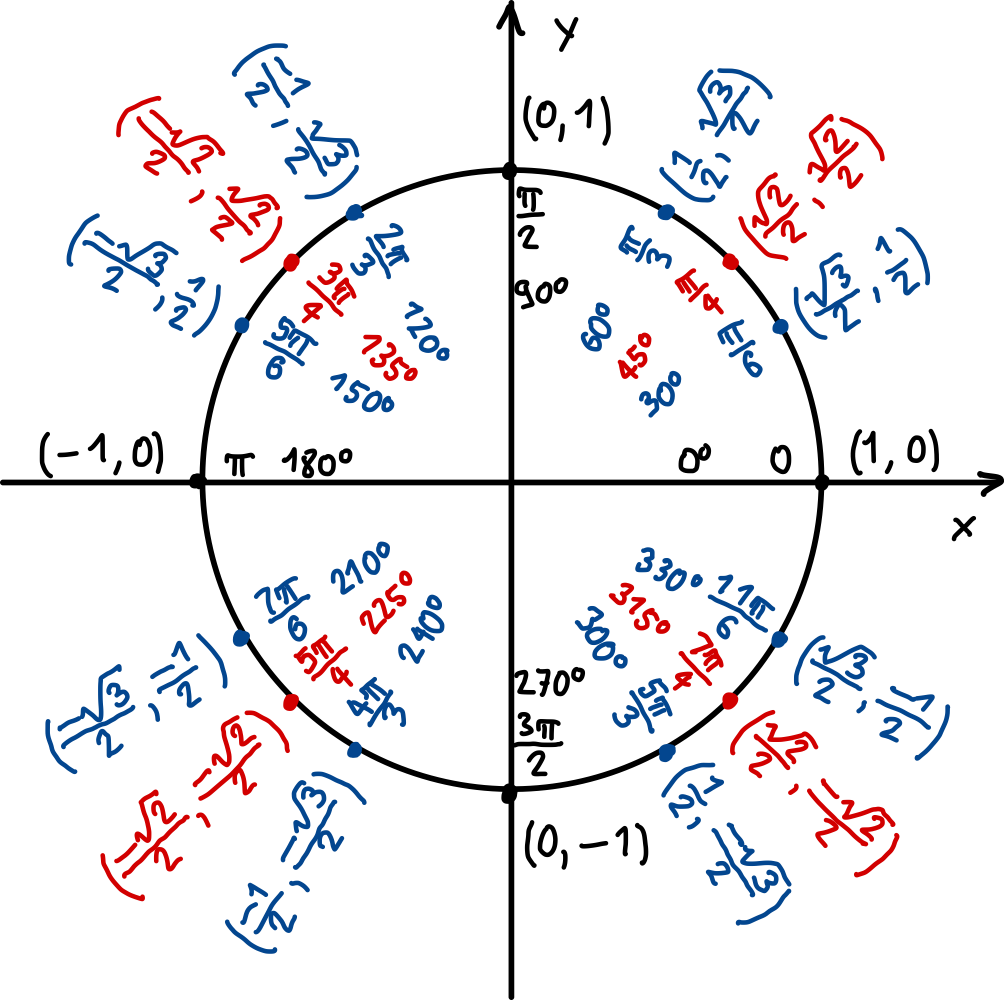
\includegraphics[width=\linewidth]{Einheitskreis.png}
  
\end{center}

\section{Tabellen}
\subsection{Ableitungen}
\begin{center}
  % the c>{\centering\arraybackslash}X is a workaround to have a column fill up all space and still be centered
  \begin{tabularx}{\linewidth}{c>{\centering\arraybackslash}Xc}
    \toprule
    $\mathbf{F(x)}$ & $\mathbf{f(x)}$ & $\mathbf{f'(x)}$ \\
    \midrule
    $\frac{x^{-a+1}}{-a+1}$ & $\frac{1}{x^a}$ & $\frac{a}{x^{a+1}}$ \\
    $\frac{x^{a+1}}{a+1}$ & $x^a \ (a \ne 1)$ & $a \cdot x^{a-1}$ \\
    $\frac{1}{k \ln(a)}a^{kx}$ & $a^{kx}$ & $ka^{kx} \ln(a)$ \\
    $\ln |x|$ & $\frac{1}{x}$ & $-\frac{1}{x^2}$ \\
    $\frac{2}{3}x^{3/2}$ & $\sqrt{x}$ & $\frac{1}{2\sqrt{x}}$\\
    $-\cos(x)$ & $\sin(x)$ & $\cos(x)$ \\
    $\sin(x)$ & $\cos(x)$ & $-\sin(x)$ \\
    $\frac{1}{2}(x-\frac{1}{2}\sin(2x))$ & $\sin^2(x)$ & $2 \sin(x)\cos(x)$ \\
    $\frac{1}{2}(x + \frac{1}{2}\sin(2x))$ & $\cos^2(x)$ & $-2\sin(x)\cos(x)$ \\
    \multirow{2}*{$-\ln|\cos(x)|$} & \multirow{2}*{$\tan(x)$} & $\frac{1}{\cos^2(x)}$  \\
    & & $1 + \tan^2(x)$ \\
    $\cosh(x)$ & $\sinh(x)$ & $\cosh(x)$ \\
    $\log(\cosh(x))$ & $\tanh(x)$ & $\frac{1}{\cosh^2(x)}$ \\
    $\ln | \sin(x)|$ & $\cot(x)$ & $-\frac{1}{\sin^2(x)}$ \\
    $\frac{1}{c} \cdot e^{cx}$ & $e^{cx}$ & $c \cdot e^{cx}$ \\
    $x(\ln |x| - 1)$ & $\ln |x|$ & $\frac{1}{x}$ \\
    $\frac{1}{2}(\ln(x))^2$ & $\frac{\ln(x)}{x}$ & $\frac{1 - \ln(x)}{x^2}$ \\
    $\frac{x}{\ln(a)} (\ln|x| -1)$ & $\log_a |x|$ & $\frac{1}{\ln(a)x}$ \\
    \bottomrule
  \end{tabularx}
\end{center}
\subsection{Weitere Ableitungen}
\begin{center}
  \begin{tabularx}{\linewidth}{>{\centering\arraybackslash}X>{\centering\arraybackslash}X}
    \toprule
    $\mathbf{F(x)}$ & $\mathbf{f(x)}$ \\
    \midrule
    $\arcsin(x)$ & $\frac{1}{\sqrt{1 - x^2}}$ \\
    $\arccos(x)$ & $\frac{-1}{\sqrt{1 - x^2}}$ \\
    $\arctan(x)$ & $\frac{1}{1 + x^2}$ \\ 
    $x^x \ (x > 0)$ & $x^x \cdot (1 + \ln x)$ \\
    \bottomrule
  \end{tabularx}
\end{center}
\subsection{Integrale}
\begin{center}
  \begin{tabularx}{\linewidth}{>{\centering\arraybackslash}X>{\centering\arraybackslash}X}
    \toprule
    $\mathbf{f(x)}$ & $\mathbf{F(x)}$ \\
    \midrule
    $\int f'(x) f(x) \dx$ & $\frac{1}{2}(f(x))^2$ \\
    $\int \frac{f'(x)}{f(x)} \dx$ & $\ln|f(x)|$ \\
    $\int_{-\infty}^\infty e^{-x^2} \dx$ & $\sqrt{\pi}$ \\
    $\int (ax+b)^n \dx$ & $\frac{1}{a(n+1)}(ax+b)^{n+1}$ \\
    $\int x(ax+b)^n \dx$ & $\frac{(ax+b)^{n+2}}{(n+2)a^2} - \frac{b(ax+b)^{n+1}}{(n+1)a^2}$ \\
    $\int (ax^p+b)^n x^{p-1} \dx$ & $\frac{(ax^p+b)^{n+1}}{ap(n+1)}$ \\
    $\int (ax^p + b)^{-1} x^{p-1} \dx$ & $\frac{1}{ap} \ln |ax^p + b|$ \\
    $\int \frac{ax+b}{cx+d} \dx$ & $\frac{ax}{c} - \frac{ad-bc}{c^2} \ln |cx +d|$ \\
    $\int \frac{1}{x^2+a^2} \dx$ & $\frac{1}{a} \arctan \frac{x}{a}$ \\
    $\int \frac{1}{x^2 - a^2} \dx$ & $\frac{1}{2a} \ln\left| \frac{x-a}{x+a} \right|$ \\
    $\int \sqrt{a^2+x^2} \dx $ & $\frac{x}{2}f(x) + \frac{a^2}{2}\ln(x+f(x))$ \\
    \bottomrule
  \end{tabularx}
\end{center}

% end of larger array spacing
\endgroup
\section{Aufgaben}
\subsection{Wahr-Falsch-Aufgaben}
\begin{enumerate}
    \item The function $x \mapsto \frac{1}{1 + x^2}$ is a solution of the differential equation $x^2y' + 2xy + y' = 0$. \textbf{True}
    \item The function $f: \R^2 \rightarrow \R$ given by
    \[f(x,y) = 
    \begin{cases}
        \frac{x^2 - y^2}{x^2 + y^2} &\text{if } (x, y) \neq (0, 0)\\
        0 &\text{if } (x, y) = (0, 0)
    \end{cases}
    \]
    is \textbf{not} continuous at $(0, 0)$. \textbf{True}
    \item Although $\lim_{(x, y) \to (0, 0)} \sin \left(\frac{1}{x^2 + |y|}\right)$ does not exist, the limit
    \[\lim_{(x, y) \to (0, 0)} x^4 \sin \left(\frac{1}{x^2 + |y|}\right)\]
    exists and is finite. \textbf{True}
    \item There exists a function $f: \R^2 \to \R$ so that for every point $(x, y) \in \R^2$, the gradient of $f$ at $(x, y)$ is equal to $(-y, x)$. \textbf{False}
    \item Let
    \[F(x, y) = (F_1, F_2)(x, y) = \left(\frac{-y}{x^2 + y^2}, \frac{x}{x^2 + y^2}\right)\]
    and let $\gamma$ be the standard parametrization of the unit circle centered at the origin and oriented counter-clockwise. Since $\pdv{F_2}{x} = \pdv{F_1}{y}$, by Green's theorem it holds that $\int_\gamma F \cdot d \Vec{s} = 0$. \textbf{False}
    \item If all the first order partial derivatives of a differentiable function $f: \R^2 \to \R$ vanish at the point $(1, 2)$, then $(1, 2)$ is a local minimum or local maximum of $f$. \textbf{False}
    \item It holds that
    \[\int_0^1 \int_0^{3x} e^{x^2} \mathop{dy} \mathop{dx} = \int_0^3 \int_{\frac{y}{3}}^1 e^{x^2} \mathop{dx} \mathop{dy} \text{.}\]
    \textbf{True}
    \item Let $f: \R^2 \to \R$ be a smooth function such that its gradient at the point $(3, 4)$, $\nabla f(3, 4)$, is equal to $(5, 6)$. Then:
    \begin{enumerate}
        \item $f$ increases at $(3, 4)$ the most in the direction of the vector $(5, 6)$. \textbf{True}
        \item The directional derivative of $f$ at the point $(3, 4)$ in the direction of the vector $\left(\frac{1}{\sqrt{2}}, \frac{1}{\sqrt{2}}\right)$ is equal to $\frac{7}{\sqrt{2}}$. \textbf{False}
        \item If $\gamma$ parametrizes some curve in $\Gamma = \{(x, y): f(x, y) = f(3, 4)\}$, then $\left.\mathop{\frac{d}{dt}} (f(\gamma(t))\right|_{t = 0} = (5, 6) \cdot \gamma(0)$. \textbf{False}
    \end{enumerate}
\end{enumerate}
\subsection{Kurzfragen}
\begin{enumerate}
    \item \textbf{Q: } Evaluate the double integral
    \[\int \int_A \frac{\log \sqrt{x^2 + y^2}}{x^2 + y^2} \mathop{dx} \mathop{dy} \text{,}\]
    where $A$ is the annulus $A = \{(x, y) \in \R^2: 1 \le x^2 + y^2 \le 4\}$.\\
    \textbf{A:} $\pi (\log 2)^2$. In polar coordinates we obtain:
    \begin{multline*}
        \int_D \frac{\log \sqrt{x^2 + y^2}}{x^2 + y^2} \mathop{dx} \mathop{dy} = \int_0^{2 \pi} \int_1^2 \frac{\log r}{r^2} r \mathop{dr} \mathop{d \theta}\\
        = 2 \pi \int_1^2 \frac{\log r}{r} \mathop{dr} = \pi \left[(\log r)^2\right]_1^2 \text{.}
    \end{multline*}
    \item \textbf{Q:} Let $g: \R^2 \to \R$ be a smooth function so that
    \[\nabla g(1, 1, \sqrt{2}) = (3, 2, -1) \text{.}\]
    Compute
    \[\pdv{g}{\phi} (\rho, \theta, \phi) \text{ at } (\rho, \theta, \phi) = \left(2, \frac{\pi}{4}, \frac{\pi}{4}\right) \text{,}\]
    where $x = \rho \cos \theta \sin \phi$, $y = \rho \sin \theta \sin \phi$ and $z = \rho \cos \phi$ are the spherical coordinates.\\
    \textbf{A:} $5 + \sqrt{2}$. As a consequence of the chain rule, we have
    \begin{align*}
        &\pdv{g}{\phi} (\rho, \theta, \phi)\\
        = &\pdv{}{\phi} \bigl(g(\rho \cos \theta \sin \phi,\, \rho \sin \theta \sin \phi,\, \rho \cos \phi)\bigr)\\
        = &\pdv{g}{x} \rho \cos \theta \cos \phi + \pdv{g}{y} \rho \sin \theta \cos \phi - \pdv{g}{z} \rho \sin \phi \text{.}
    \end{align*}
    Since
    \begin{multline*}
        \bigl(2 \cos \left(\frac{\pi}{4}\right) \sin \left(\frac{\pi}{4}\right),\,\bigr.\\
        \bigl.2 \sin \left(\frac{\pi}{4}\right) \sin \left(\frac{\pi}{4}\right),\, 2 \cos \left(\frac{\pi}{4}\right)\bigr) = (1, 1, \sqrt{2}) \text{,}
    \end{multline*}
    we then deduce
    \begin{align*}
        &\pdv{g}{\phi} \left(2, \frac{\pi}{4}, \frac{\pi}{4}\right)\\
        =& 3 \cdot 2 \cos \left(\frac{\pi}{4}\right) \cos \left(\frac{\pi}{4}\right) + 2 \cdot \sin \left(\frac{\pi}{4}\right) \cos \left(\frac{\pi}{4}\right) + 1 \cdot 2 \cos \left(\frac{\pi}{4}\right)\\
        =& 5 + \sqrt{2} \text{.}
    \end{align*}
    \item \textbf{Q:} Evaluate the double integral
    \[\int \int_R \frac{\sin x}{x} \mathop{dx} \mathop{dy} \text{,}\]
    where $R$ is the triangle in the $xy$-plane bounded by the $x$-axis and the lines $y = 2x$ and $x = \frac{\pi}{4}$.\\
    \textbf{A:} $2 - \sqrt{2}$. The domain $R$ is defined by $0 \le x \le \frac{\pi}{4}$ and $0 \le y \le 2x$, thus the integral is
    \begin{multline*}
        \int_0^{\frac{\pi}{4}} \int_0^{2x} \frac{\sin x}{x} \mathop{dy} \mathop{dx} = \int_0^{\frac{\pi}{4}} \frac{\sin x}{x} 2x \mathop{dx}\\
        = 2 \left[- \cos x\right]_0^{\frac{\pi}{4}} = 2 - \sqrt{2} \text{.}
    \end{multline*}
    \item \textbf{Q:} What is the line integral of the vector field
    \[F: \R^2 \to \R^2,\; F(x, y) = (1 - y + 2xy,\, x^2 + y^2) \text{,}\]
    along the boundary of the region between the circle of radius $2$ and the triangle whose vertices are at $(0, 0)$, $(1, 0)$ and $(0, 1)$? The boundary is oriented so that the region is to the left.\\
    \textbf{A:} $4 \pi - \frac{1}{2}$. Since $\curl F = 1$, by Green's theorem we get
    \begin{multline*}
        \int_{\partial R} F \cdot d \Vec{s} = - \int_R \mathop{dx} \mathop{dy}\\
        = \text{Area}(\text{Disk}) - \text{Area}(\text{Triangle}) = 4 \pi - \frac{1}{2} \text{.}
    \end{multline*}
    \item \textbf{Q:} Let $f: \R^2 \to \R$ be the function given by
    \[f(x, y) = 1 + ye^{xy} \text{.}\]
    Find the best approximating affine function $A: \R^2 \to \R$ (that is, $A = a_0 + L$ where $a_0$ is a constant and $L: \R^2 \to \R$ is linear) for $f$ at the point $(2, 0)$.\\
    \textbf{A:} $1 + y$. The theory tells that A is given by the 1st order Taylor polynomial:
    \begin{align*}
        &A(x, y)\\
        =& f(2, 0) + \partial_x f(2, 0) x + \partial_y f(2, 0) y\\
      =& 1 + \left[y^2 e^{xy}\right]_{(x, y) = (2, 0)} x + \left[(1 + xy) e^{xy}\right]_{(x, y) = (2, 0)} y\\
      =& 1 + y \text{.}
    \end{align*}
\end{enumerate}
\subsection{Probleme}
\begin{enumerate}
    \item Consider the differential equation
    \[y'' - y' + y = (t + 1) e^t \text{.} \tag{\star}\]
    \begin{enumerate}
        \item \textbf{Q:} Find the general solution of the homogeneous equation associated to $(\star)$.\\
        \textbf{A:} The characteristic polynomial is $\lambda^2 - \lambda + 1$, whose roots are $\frac{1 \pm \sqrt{3}i}{2}$. Consequently the general solution of the homogeneous equation is
        \[y_h(t) = e^{\frac{1}{2}t} \left(C_1 \cos \left(\frac{\sqrt{3}}{2} t\right) + C_2 \sin \left(\frac{\sqrt{3}}{2} t\right)\right) \text{.}\]
        \item \textbf{Q:} Find the general solution of $(\star)$.\\
        \textbf{A:} We just need to find a particular solution. Since $1$ is not a root of the characteristic polynomial, we make the Ansatz
        \[y_p(t) = (At + B) e^t \text{.}\]
        Substituting this in the equation one finds that
        \[At + A + B \overset{!}{=} t + 1 \text{,}\]
        hence $A = 1$ and $B = 0$. Thus the general solution is
        \begin{multline*}
            y(t) = y_h(t) + t_p(t) =\\
            e^{\frac{1}{2} t} \left(C_1 \cos \left(\frac{\sqrt{3}}{2} t \right) + C_2 \sin \left(\frac{\sqrt{3}}{2} t\right)\right) + te^t \text{.}
        \end{multline*}
        \item \textbf{Q:} Find the solution of $(\star)$ satisfying the conditions $y(0) = 0,\, y'(0) = 1$.\\
        \textbf{A:} Replacing the given conditions in the above formula yields
        \begin{align*}
            y(0) = 0 &\implies C_1 = 0,\\
            y'(0) = 0 &\implies C_2 = 0 \text{,}
        \end{align*}
        which means that the required solution is $y(t) = te^t$.
    \end{enumerate}
    \item Let $f: \R^2 \to \R$ be given by
    \[f(x, y) = x^4 + y^4 - 2x^2 -2y^2 + 2 \text{.}\]
    \begin{enumerate}
        \item \textbf{Q:} Determine the critical points of $f$ and their type (local min, local max, saddle).\\
        \textbf{A:} We have
        \begin{align*}
            \pdv{f}{x}(x, y) &= 4x^3 - 4x,\\
            \pdv{f}{y}(x, y) &= 4y^3 - 4y \text{.}
        \end{align*}
        Hence the critical points are determined by
        \[
        \begin{cases}
            x(x^2 - 1) = 0\\
            y(y^2 - 1) = 0 \text{,}
        \end{cases}
        \]
        and thus are 9:
        \[(0, 0),\, (\pm 1, 0),\, (0, \pm 1),\, (\pm 1, \pm 1) \text{,}\]
        with all possible choices of sign. The Hessian of $f$ is
        \[\Hess f(x, y) =
        \begin{pmatrix*}
            12 x^2 - 4 & 0\\
            0 & 12 y^2 - 4
        \end{pmatrix*}
        \text{,}\]
        consequently
        \begin{align*}
            \Hess f(0, 0) &=
            \begin{pmatrix*}
                -4 & 0\\
                0 & -4
            \end{pmatrix*}
            ,\,\\
            \Hess f(\pm 1, 0) &=
            \begin{pmatrix*}
                8 & 0\\
                0 & -4
            \end{pmatrix*}
            ,\,\\
            \Hess f(0, \pm 1) &=
            \begin{pmatrix}
                -4 & 0\\
                0 & 8
            \end{pmatrix}
            ,\,\\
            \Hess f(\pm 1, \pm 1) &=
            \begin{pmatrix*}
                8 & 0\\
                0 & 8
            \end{pmatrix*}
            \text{,}
        \end{align*}
        and so we see that $(0, 0)$ is a local maximum, $(\pm 1, \pm 1)$ are local minima and $(0, \pm 1)$, $(\pm 1, 0)$ are saddles.
        \item \textbf{Q:} Does $f$ attain global maximum and global minimum? If so, at which points?\\
        \textbf{A:} Since
        \[\lim_{(x, y) \to \infty} f(x, y) = +\infty \text{,}\]
        $f$ does not have a global maximum.
        For the same reason however, (or because $f \ge 0$ and $f(\pm 1, \pm 1) = 0$) it must attain its global minimum and thus from the above this is attained at the points $(\pm 1, \pm 1)$.
    \end{enumerate}
    \item Consider the integral
    \[\int \int_D (y - x)^2 (x + y)^{2020} \mathop{dx} \mathop{dy} \text{,}\]
    where $D$ is the region bounded by the coordinate axes and the line $x + y = 2$.
    \begin{enumerate}
        \item \textbf{Q:} Consider the change of variables defined by
        \[u = y - x \text{ and } v = x + y \text{.}\]
        Find the region $R$ in the $uv$-plane which corresponds to $D$ in the $xy$-plane.\\
        \textbf{A:} The inverse of the transformation is given by
        \[x = \frac{1}{2} (-u + v) \text{ and } y = \frac{1}{2} (u + v) \text{,}\]
        Thus, since $D$ is defined by
        \[
        \begin{cases}
            0 \le x \le 2,\\
            0 \le y \le 2 - x \text{,}
        \end{cases}
        \]
        we deduce that $R$ is expressed as
        \[
        \begin{cases}
            u + v \le u - v + 4,\\
            -u + v \ge 0,\\
            -u + v \le 4,\\
            u + v \ge 0
        \end{cases}
        \iff
        \begin{cases}
            v \le 2,\\
            v \ge u,\\
            v \le u + 4,\\
            v \ge -u \text{,}
        \end{cases}
        \]
        which we may rewrite as
        \[
        \begin{cases}
            0 \le v \le 2,\\
            -v \le u \le v \text{.}
        \end{cases}
        \]
        \item \textbf{Q:} Evaluate the above integral using the change of variables given in $(a)$.\\
        \textbf{A:} Since the determinant of the Jacobi matrix of the transformation is $- \frac{1}{2}$, the integral becomes
        \begin{align*}
            &\int \int_D (x - y)^2 (x + y)^{2020} \mathop{dx} \mathop{dy}\\
            = &\frac{1}{2} \int \int_R u^2v^{2020} \mathop{du} \mathop{dv}\\
            = &\frac{1}{2} \left(\int_0^2 v^{2020} \left[\frac{u^3}{3}\right]_{-v}^v \mathop{du}\right) = \frac{1}{3} \int_0^2 v^{2023} \mathop{du} = \frac{2^2024}{3 \cdot 2024} \text{.}
        \end{align*}
    \end{enumerate}
    \item Let $F: \R^3 \to \R^3$ be the vector field given by
    \[F(x, y, z) = (z \cos x,\, 1 + z^2e^{yz^2},\,\sin x + 2yze^{yz^2}) \text{.}\]
    \begin{enumerate}
        \item \textbf{Q:} Show that $F$ is conservative.\\
        \textbf{A:} One checks directly that
        \[\pdv{}{x_i} F_j = \pdv{}{x_j} F_i\; \text{for } i, j = 1, 2, 3 \text{,}\]
        hence since $\R^3$ is star-shaped, $F$ is conservative.
        \item \textbf{Q:} Find a potential $g: \R^3 \to \R$ for $F$.\\
        \textbf{A:} The function $g$ needs to be so that
        \begin{align*}
            \pdv{}{x} g &= z \cos x,\\
            \pdv{}{y} g &= 1 + z^2 e^{yz^2},\\
            \pdv{}{z} g &= \sin x + 2yze^{yz^2} \text{.}
        \end{align*}
        A moment of thought yields that one such $g$ is
        \[g(x, y, z) = z \sin x + y + e^{yz^2} \text{.}\]
        \item \textbf{Q:} Find the value of the line integral $\int_\gamma F \cdot d \Vec{s}$, where $\gamma: [0, \pi] \to \R^3$ is the coil-shaped curve given by
        \begin{multline*}
            \gamma(t) = (\sin(200t),\, (2 + \cos(200t)) \cos(t),\,\\
            (2 + \cos(200t)) \sin(t)) \text{.}
        \end{multline*}\\
        \textbf{A:} Since $F$ is conservative, with (b) we get that
        \begin{multline*}
            \int_\gamma F \cdot d \Vec{s} = g(\gamma(\pi)) - g(\gamma(0))\\
            = g(0, -3, 0) - g(0, 3, 0) = -6 \text{.}
        \end{multline*}
    \end{enumerate}
\end{enumerate}
\section{Quellen}
Ein Grossteil des Cheatsheets wurde stark vom Cheatsheet von \href{https://github.com/dannycamenisch}{Danny Camenisch} inspiriert. Ausserdem stammen Teile der Tabellen aus dem Buch ``Formeln, Tabellen und Konzepte''. Die Definitionen sind meistens dem Skript ``Analysis 1'' von Marc Burger und dem Skript ``Analysis 2'' von E. Kowalski entnommen.
\end{document}
